\documentclass[a4paper,11pt,oneside]{book}

% Font và tiếng Việt
\usepackage[utf8]{vietnam}
\usepackage{listings}
\usepackage{xcolor}
\usepackage{setspace}
\setstretch{1.3}

% Toán học
\usepackage{amsmath,amssymb,amsthm,amsfonts,mathtools}

% Căn lề
\usepackage[left=3cm,right=2cm,top=2.5cm,bottom=3cm,footskip=40pt]{geometry}
\setlength{\parindent}{0cm}
\setlength{\parskip}{0.6ex}
\usepackage{indentfirst}

% Hình ảnh
\usepackage{graphicx}
\graphicspath{{figures/}} % thư mục chứa ảnh
\usepackage{caption}
\usepackage{subfigure}

% Vẽ
\usepackage{tikz}
\usetikzlibrary{calc,arrows,positioning,shapes}

% Bảng
\usepackage{booktabs}
\usepackage{multirow}
\usepackage{array}
\usepackage{tabularx}
\newcolumntype{C}[1]{>{\centering\arraybackslash}m{#1}}

% Danh mục mục lục, hình, bảng
\usepackage[subfigure]{tocloft}

\usepackage{enumitem}
\setlist[itemize]{label=\textbullet, leftmargin=1.5em}
\usepackage{float}
\usepackage{placeins}
\renewcommand{\cftfigfont}{Hình~}
\renewcommand{\cfttabfont}{Bảng~ }
\renewcommand{\labelitemi}{\textbullet}

% Chương, tiêu đề
\usepackage{titlesec}
\titleformat{\chapter}[display] 
  {\fontsize{14}{16}\selectfont\bfseries\centering}
  {\MakeUppercase{\chaptertitlename}\ \thechapter}{0pt}{\fontsize{14}{16}\selectfont\MakeUppercase}
\titlespacing{\chapter}{0pt}{0pt}{40pt} 
\titleformat*{\section}{\fontsize{14}{14}\selectfont\bfseries}
\titleformat*{\subsection}{\fontsize{14}{14}\selectfont\bfseries\slshape}

% Trích dẫn
\usepackage[square,comma,numbers,sort&compress]{natbib}
\bibliographystyle{IEEEtran}

% Liên kết
\usepackage[hidelinks,unicode]{hyperref}

\captionsetup[table]{position=bottom}
\captionsetup[figure]{skip=10pt}



% Định nghĩa, định lý
\newtheorem{definition}{\bf Định nghĩa}[chapter]
\newtheorem{theorem}{\bf Định lý}[chapter]
\newtheorem{lemma}{\bf Bổ đề}[chapter]

% Listing settings
\lstset{
  basicstyle=\ttfamily\small,
  backgroundcolor=\color{gray!10},
  frame=single,
  keywordstyle=\color{blue},
  commentstyle=\color{green!50!black},
  stringstyle=\color{orange},
  showstringspaces=false,
  breaklines=true,
  numbers=left,
  numberstyle=\tiny\color{gray}
}

% Algorithm
\usepackage{algorithm}
\floatname{algorithm}{Thuật toán}
\usepackage{algpseudocode}

\begin{document}
\fontsize{11}{13.2}\selectfont

% ========================
% Các phần cover
% ========================
\pagestyle{empty}
\begin{titlepage}

\begin{tikzpicture}[remember picture, overlay]
  \draw[line width = 2pt] ($(current page.north west) + (1in,-1in)$) rectangle ($(current page.south east) + (-0.5in,1in)$);
\end{tikzpicture}

\begin{center}

\vspace*{0.5cm}

{\Large \textbf{ĐẠI HỌC QUỐC GIA HÀ NỘI}}

{\Large \textbf{TRƯỜNG ĐẠI HỌC CÔNG NGHỆ}}

\vspace{20mm}


\includegraphics[width=0.25\linewidth]{figures/uet.png}

\vspace{3mm}

\noindent
{\Large \textbf{BÁO CÁO DỰ ÁN CÔNG NGHỆ\\}}
{\Large \textbf{Ngành: Khoa học máy tính\\}}

\smallskip
\vspace{10mm}

{\LARGE \textbf{HỆ THỐNG TỰ ĐỘNG CÂN BẰNG GAME ROGUELIKE DECKBUILDER SỬ DỤNG THUẬT TOÁN DI TRUYỀN}}

\bigskip

\end{center}

\vspace{15mm}

\centering
\begin{spacing}{0.8}
\begin{tabular}{ll}
Giảng viên hướng dẫn:  & TS. Lê Nguyên Khôi \\[1ex]
Sinh viên thực hiện:   & Nguyễn Nhật Phong \\[1ex]
Mã sinh viên:          & 22028272 \\[1ex]
Lớp:                   & QH-2022-I/CQ-I-CS2
\end{tabular}
\end{spacing}

\vspace{15mm}

\begin{center}
\textbf{HÀ NỘI - 2025}
\end{center}

\end{titlepage}

\newpage
\begin{titlepage}
\begin{center}

\vspace*{1cm}

{\large \textbf{ĐẠI HỌC QUỐC GIA HÀ NỘI}}

{\large \textbf{TRƯỜNG ĐẠI HỌC CÔNG NGHỆ}}

\vspace{2cm}

{\Large \textbf{BÁO CÁO DỰ ÁN CÔNG NGHỆ}}

\vspace{1cm}

{\LARGE \textbf{HỆ THỐNG TỰ ĐỘNG CÂN BẰNG GAME ROGUELIKE DECKBUILDER SỬ DỤNG THUẬT TOÁN DI TRUYỀN}}

\vspace{0.5cm}

{\large \textit{Automatic Game Balancing System for Roguelike Deckbuilder\\
Using Genetic Algorithms}}

\vspace{3cm}

\centering
\begin{spacing}{0.8}
\begin{tabular}{ll}
Giảng viên hướng dẫn:  & TS. Lê Nguyên Khôi \\[1ex]
Sinh viên thực hiện:   & Nguyễn Nhật Phong \\[1ex]
Mã sinh viên:          & 22028272 \\[1ex]
Lớp:                   & QH-2022-I/CQ-I-CS2
\end{tabular}
\end{spacing}

\vfill

{\large HÀ NỘI - 2025}

\end{center}
\end{titlepage}

\newpage

% ========================
% Mục lục
% ========================
\pagenumbering{roman}
\renewcommand{\contentsname}{\vspace{-70pt}\centerline{\fontsize{14}{16}\selectfont\MakeUppercase{Mục lục}}}
\tableofcontents
\newpage

% ========================
% Các phần đầu
% ========================
\setcounter{page}{1}
\chapter*{LỜI CAM ĐOAN}
\addcontentsline{toc}{chapter}{Lời cam đoan}

\vspace{1cm}

Em xin cam đoan đây là công trình nghiên cứu của riêng em. Các kết quả nghiên cứu và các kết luận trong đề tài này là trung thực, không sao chép từ bất kỳ nguồn nào và dưới bất kỳ hình thức nào. Việc tham khảo các nguồn tài liệu (nếu có) đã được thực hiện trích dẫn và ghi nguồn đầy đủ theo đúng quy định.

Nếu phát hiện có bất kỳ gian lận nào, em xin hoàn toàn chịu trách nhiệm về nội dung đề tài của mình. Trường Đại học Công nghệ không liên quan đến những vi phạm tác quyền, bản quyền do em gây ra trong quá trình thực hiện (nếu có).

\vspace{3cm}

\begin{flushright}
Hà Nội, ngày 18 tháng 12 năm 2025\\
Sinh viên thực hiện\\
\vspace{2cm}
Nguyễn Nhật Phong
\end{flushright}

\newpage
\chapter*{LỜI CẢM ƠN}
\addcontentsline{toc}{chapter}{Lời cảm ơn}

\vspace{1cm}

Để hoàn thành đề tài "Hệ thống tự động cân bằng game Roguelike Deckbuilder sử dụng thuật toán di truyền", em xin chân thành cảm ơn:

Thầy TS. Lê Nguyên Khôi, giảng viên hướng dẫn, đã tận tình chỉ bảo, động viên và định hướng em trong suốt quá trình thực hiện đề tài. Những góp ý quý báu của Thầy đã giúp em hoàn thiện cả về mặt kỹ thuật lẫn cách tiếp cận nghiên cứu.

Các thầy cô trong Khoa Công nghệ thông tin, Trường Đại học Công nghệ, Đại học Quốc gia Hà Nội đã truyền đạt kiến thức nền tảng vững chắc về lập trình, thuật toán, tạo tiền đề quan trọng cho đề tài này.

Các bạn sinh viên đã tham gia playtesting và đóng góp feedback quý báu cho hệ thống.

Em xin chân thành cảm ơn!

\vspace{2cm}

\begin{flushright}
Hà Nội, ngày 18 tháng 12 năm 2025\\
Sinh viên thực hiện\\
\vspace{2cm}
Nguyễn Nhật Phong
\end{flushright}
 
\newpage
\chapter*{TÓM TẮT}
\addcontentsline{toc}{chapter}{Tóm tắt}

\vspace{0.5cm}

\noindent\textbf{Từ khóa:} Game Balancing, Thuật toán di truyền, NSGA-II, Roguelike Deckbuilder, Tối ưu hóa đa mục tiêu, Procedural Content Generation

\vspace{1cm}

Cân bằng game (game balancing) là một thách thức lớn trong phát triển trò chơi điện tử, đặc biệt với thể loại Roguelike Deckbuilder nơi mỗi lượt chơi là độc nhất với các yếu tố ngẫu nhiên. Phương pháp truyền thống dựa vào kinh nghiệm và thử nghiệm thủ công tốn nhiều thời gian và dễ bỏ sót các kịch bản quan trọng.

Đề tài này nghiên cứu và phát triển một hệ thống tự động cân bằng game sử dụng thuật toán di truyền (Genetic Algorithm - GA). Hệ thống bao gồm: (1) một Roguelike Deckbuilder prototype hoàn chỉnh với hệ thống chiến đấu, quản lý bộ bài, sinh bản đồ và hệ thống di vật; (2) AI agent tự động chơi game để thu thập dữ liệu; (3) hai phương pháp tối ưu hóa: GA đơn mục tiêu với GA truyền thống tối ưu \~{}500 tham số và NSGA-II đa mục tiêu tối ưu \~{}50 tham số phân cấp.

Thực nghiệm với 30 thế hệ và 100 cá thể mỗi thế hệ cho thấy phương pháp NSGA-II đa mục tiêu vượt trội hơn: tiết kiệm 33\% thời gian tính toán (49 phút so với 73 phút), tăng Balance Score từ 0.754 lên 0.960 (+27.3\%), Engagement Score từ 0.655 lên 0.900 (+37.4\%), và đạt Coherence score tối đa 1.000 (+17.2\%). Phương pháp này tìm được Pareto front gồm nhiều giải pháp không bị chi phối, cho phép người dùng chọn sự đánh đổi phù hợp giữa Balance, Engagement và Coherence. Số lượng thẻ bài khả dụng tăng 16.7\% (12 lên 14) và Build Variety tăng 34.8\% (0.705 lên 0.950).

Hệ thống chứng minh hiệu quả của việc kết hợp kiến thức chuyên môn (gom nhóm tham số phân cấp) với tối ưu hóa đa mục tiêu trong cân bằng game. Công cụ có tiềm năng lớn để tự động hóa quá trình cân bằng, tiết kiệm hàng trăm giờ điều chỉnh thủ công cho các nhà phát triển game.

\newpage
\addcontentsline{toc}{chapter}{Danh mục hình vẽ}
\listoffigures
\newpage
\addcontentsline{toc}{chapter}{Danh mục bảng biểu}
\listoftables
\newpage
\clearpage
\phantomsection
\chapter*{DANH MỤC CÁC KÝ HIỆU VÀ CHỮ VIẾT TẮT}
\addcontentsline{toc}{chapter}{Danh mục các ký hiệu và chữ viết tắt}

\section*{Chữ viết tắt}
\begin{tabularx}{\textwidth}{l X}
    \textbf{AI} & Artificial Intelligence - Trí tuệ nhân tạo \\
    \textbf{GA} & Genetic Algorithm - Thuật toán di truyền \\
    \textbf{NSGA-II} & Non-dominated Sorting Genetic Algorithm II - Thuật toán di truyền sắp xếp không bị chi phối phiên bản 2 \\
    \textbf{MOEA/D} & Multi-Objective Evolutionary Algorithm based on Decomposition \\
    \textbf{PCG} & Procedural Content Generation - Sinh nội dung tự động \\
    \textbf{HP} & Health Points - Điểm sinh mạng \\
    \textbf{MOBA} & Multiplayer Online Battle Arena \\
    \textbf{PPO} & Proximal Policy Optimization \\
    \textbf{DQN} & Deep Q-Network \\
    \textbf{RPG} & Role-Playing Game - Trò chơi nhập vai \\
    \textbf{SBX} & Simulated Binary Crossover - Lai ghép nhị phân mô phỏng \\
\end{tabularx}

\vspace{1cm}

\section*{Ký hiệu toán học}
\begin{tabularx}{\textwidth}{l X}
    $G$ & Không gian genome (genome space) \\
    $f$ & Hàm fitness \\
    $f_i$ & Hàm mục tiêu thứ $i$ \\
    $F(x)$ & Vector các hàm mục tiêu đa chiều \\
    $x$ & Một giải pháp (genome) \\
    $x_1 \prec x_2$ & Giải pháp $x_1$ Pareto dominant giải pháp $x_2$ \\
    $p_m$ & Tỷ lệ đột biến (mutation rate) \\
    $\sigma$ & Độ lệch chuẩn của phân phối Gaussian \\
    $\mathcal{N}(0, \sigma)$ & Phân phối Gaussian với trung bình 0 và độ lệch chuẩn $\sigma$ \\
    $P(i)$ & Xác suất chọn cá thể thứ $i$ \\
    $N$ & Kích thước quần thể (population size) \\
    $m$ & Số lượng mục tiêu (number of objectives) \\
    $d_i$ & Crowding distance của giải pháp thứ $i$ \\
    $f_k^{\max}, f_k^{\min}$ & Giá trị lớn nhất và nhỏ nhất của mục tiêu $k$ \\
    $w_i$ & Trọng số của metric/objective thứ $i$ \\
    $\alpha, \beta, \lambda$ & Các hệ số cân bằng trong hàm fitness \\
    $\Delta_{wr}, \Delta_{hp}, \Delta_{fd}$ & Độ lệch win rate, victory HP, floor on death \\
    $\alpha_{wr}, \alpha_{hp}, \alpha_{fd}$ & Hệ số độ nhạy (sensitivity) cho các metrics \\
\end{tabularx}

\clearpage
\vspace{1cm}

\section*{Thuật ngữ chuyên ngành}
\begin{tabularx}{\textwidth}{l X}
    \textbf{Pareto Front} & Tập hợp các giải pháp Pareto optimal (không bị chi phối) \\
    \textbf{Genome} & Nhiễm sắc thể, đại diện cho một giải pháp trong GA \\
    \textbf{Gene} & Gen, một tham số đơn lẻ trong genome \\
    \textbf{Fitness} & Độ thích nghi, chỉ số đánh giá chất lượng giải pháp \\
    \textbf{Crossover} & Lai ghép, toán tử kết hợp hai genome cha mẹ \\
    \textbf{Mutation} & Đột biến, toán tử thay đổi ngẫu nhiên genome \\
    \textbf{Selection} & Chọn lọc, quá trình chọn genome tốt nhất \\
    \textbf{Pareto Dominance} & Quan hệ chi phối trong tối ưu đa mục tiêu \\
    \textbf{Crowding Distance} & Khoảng cách đám đông, đo mức độ đông đúc của giải pháp \\
    \textbf{Viable Cards} & Thẻ bài khả dụng, được AI chọn thường xuyên \\
    \textbf{Trap Cards} & Thẻ bài rác, được chọn nhưng có tỷ lệ thắng thấp \\
    \textbf{Build Variety} & Đa dạng lối chơi, mức độ khác biệt giữa các bộ bài thắng \\
    \textbf{Permadeath} & Khi chết phải chơi lại từ đầu, mất hết tiến độ \\
    \textbf{Synergy} & Hiệp lực, sự kết hợp hiệu quả giữa các thẻ bài \\
\end{tabularx}

\newpage

% ========================
% Nội dung chính
% ========================
\pagenumbering{arabic}
\pagestyle{plain}
\clearpage
\phantomsection
\addcontentsline{toc}{chapter}{{Mở đầu}}
\chapter*{Mở đầu}

\section{Lý do chọn đề tài}

Trong ngành công nghiệp trò chơi điện tử hiện đại, việc cân bằng gameplay là một trong những thách thức lớn nhất mà các nhà phát triển phải đối mặt. Đặc biệt với thể loại Roguelike Deckbuilder, nơi mỗi lần chơi là một trải nghiệm độc đáo với các lựa chọn ngẫu nhiên về thẻ bài, di vật và kẻ thù, việc đảm bảo game vừa thách thức vừa công bằng là cực kỳ khó khăn \cite{schell2019art}.

Phương pháp cân bằng game truyền thống thường dựa vào kinh nghiệm và thử nghiệm thủ công của các nhà thiết kế. Tuy nhiên, với số lượng lớn các tham số cần điều chỉnh (giá trị sát thương của thẻ bài, máu của kẻ địch, hiệu ứng của di vật, v.v.), phương pháp này tốn rất nhiều thời gian và có thể bỏ sót các kịch bản edge case quan trọng \cite{jaffe2012optimizing}.

Xuất phát từ thực tiễn đó, đề tài này tập trung nghiên cứu và phát triển một hệ thống cân bằng game tự động sử dụng \textbf{Thuật toán di truyền (Genetic Algorithm - GA)} để tối ưu hóa các tham số game. Hệ thống không chỉ giúp tự động hóa quá trình cân bằng mà còn có khả năng khám phá các cấu hình tối ưu mà con người có thể không nghĩ tới \cite{holland1992adaptation, yannakakis2018artificial}.

\section{Mục tiêu nghiên cứu}

Mục tiêu chính của đề tài là xây dựng một hệ thống hoàn chỉnh bao gồm việc phát triển một trò chơi Roguelike Deckbuilder prototype với đầy đủ cơ chế gameplay cơ bản, xây dựng hệ thống mô phỏng tự động có khả năng chạy hàng nghìn lượt chơi để thu thập dữ liệu, và thiết kế cùng triển khai thuật toán di truyền để tối ưu hóa các tham số game.

Bên cạnh đó, hệ thống cần so sánh hiệu quả của hai phương pháp: \textbf{GA đơn mục tiêu} (tối ưu trực tiếp từng tham số bằng GA truyền thống) và \textbf{NSGA-II đa mục tiêu} (sử dụng thuật toán NSGA-II để tối ưu đa mục tiêu với không gian tham số được cấu trúc hóa) \cite{deb2002fast, zitzler2000comparison}. Cuối cùng, đề tài phát triển công cụ trực quan hóa để phân tích kết quả và đánh giá chất lượng cân bằng đạt được.

\section{Phương pháp nghiên cứu}

Để giải quyết bài toán phức tạp nêu trên, đề tài áp dụng cách tiếp cận đa chiều kết hợp giữa nghiên cứu lý thuyết, phát triển hệ thống và tối ưu hóa thực nghiệm.

\subsection{Nghiên cứu lý thuyết}
Giai đoạn nghiên cứu lý thuyết tập trung khảo sát các thuật toán di truyền (GA) và các biến thể hiện đại như NSGA-II \cite{deb2002fast, zitzler2000comparison}, nghiên cứu các phương pháp đánh giá chất lượng cân bằng game thông qua các chỉ số như tỷ lệ thắng, điểm HP trung bình khi chiến thắng, và tầng trung bình khi thua. Đồng thời, đề tài cũng tìm hiểu về game design patterns trong thể loại Roguelike Deckbuilder, lấy cảm hứng từ các tựa game thành công như \textit{Slay the Spire} \cite{slaythespire}.

\subsection{Phát triển hệ thống}
Hệ thống được xây dựng với game engine bao gồm các module: Combat System, Deck Management, Map Generation, và Room Handlers. AI agent được thiết kế để tự động chơi game (HeuristicPlayerAI), cùng với hệ thống mô phỏng có khả năng chạy song song và ghi log đầy đủ \cite{yannakakis2018artificial}.

\subsection{Tối ưu hóa và thực nghiệm}
Quá trình tối ưu hóa được triển khai theo hai hướng tiếp cận: GA đơn mục tiêu với GA truyền thống xử lý khoảng 500 tham số, và NSGA-II đa mục tiêu chỉ cần khoảng 50 tham số phân cấp. Cả hai phương pháp đều được chạy thực nghiệm và so sánh kết quả, sau đó phân tích Pareto front để tìm các giải pháp cân bằng tối ưu \cite{preuss2012multiobjective}.

\section{Nội dung nghiên cứu}

Dự án này tập trung xây dựng một Roguelike Deckbuilder game hoàn chỉnh với các cơ chế chiến đấu theo lượt (turn-based combat), quản lý bộ bài (deck building), di vật (relics), và bản đồ phòng (room-based map) \cite{dormans2011level}. Hệ thống AI tự động chơi game được phát triển dựa trên heuristics để có thể mô phỏng hàng nghìn lượt chơi, thu thập dữ liệu về gameplay metrics.

Không gian tham số tối ưu hóa bao gồm sát thương và giá mana của thẻ bài, giá trị sức khỏe và sát thương của kẻ địch, cùng với hiệu ứng của di vật và status effects. Hàm fitness đa mục tiêu được xây dựng để đánh giá chất lượng cân bằng theo ba tiêu chí: \textbf{Balance} (độ cân bằng giữa thắng/thua), \textbf{Engagement} (độ hấp dẫn của gameplay), và \textbf{Coherence} (tính nhất quán của thiết kế) \cite{preuss2012multiobjective}.

Hai phương pháp tối ưu hóa với các chiến lược khác nhau được triển khai và so sánh, cùng với công cụ trực quan hóa để phân tích kết quả including visualizer cho Pareto front 3D và evolution charts.

\section{Đóng góp của đề tài}

Về mặt khoa học, đề tài đề xuất một mô hình tham chiếu cho việc ứng dụng thuật toán tiến hóa vào bài toán cân bằng game, đặc biệt là thể loại Roguelike Deckbuilder \cite{togelius2011search}. Nghiên cứu so sánh giữa phương pháp tối ưu trực tiếp và tối ưu phân cấp trong bối cảnh game balancing, cung cấp insights về hiệu quả của hierarchical parameter grouping.

Về mặt thực tiễn, đề tài cung cấp một công cụ hoàn chỉnh giúp các nhà phát triển game có thể tự động hóa quá trình cân bằng, tiết kiệm hàng trăm giờ thử nghiệm thủ công \cite{jaffe2012optimizing, nelson2016towards}. Hệ thống có khả năng mở rộng và có thể áp dụng cho các loại game khác với các điều chỉnh phù hợp.

Về mặt công nghệ, đề tài kiểm chứng khả năng kết hợp giữa game development và evolutionary algorithms trong một hệ thống thực tế. Công cụ trực quan hóa được phát triển giúp phân tích và hiểu sâu về quá trình tiến hóa của các tham số game, hỗ trợ game designers trong việc đưa ra quyết định thiết kế dựa trên dữ liệu khách quan \cite{smith2011analyzing}.

\section{Bố cục của báo cáo}
Báo cáo được tổ chức thành các chương chính sau:
\begin{itemize}
    \item \textbf{Mở đầu}: Trình bày bối cảnh, lý do chọn đề tài, mục tiêu và phương pháp tiếp cận.
    \item \textbf{Chương 1 - Tổng quan và Cơ sở lý thuyết}: Giới thiệu về thể loại Roguelike Deckbuilder, khảo sát các thuật toán di truyền (GA, NSGA-II), và phân tích các nghiên cứu liên quan về game balancing.
    \item \textbf{Chương 2 - Phân tích và Thiết kế hệ thống}: Mô tả kiến trúc chi tiết của game engine, hệ thống mô phỏng, và các module tối ưu hóa.
    \item \textbf{Chương 3 - Cài đặt và Triển khai}: Trình bày quy trình hiện thực hóa các module, các thách thức kỹ thuật gặp phải và giải pháp xử lý.
    \item \textbf{Chương 4 - Thực nghiệm và Đánh giá}: Phân tích kết quả chạy thực nghiệm với cả hai phương pháp tối ưu hóa, so sánh hiệu quả và đánh giá chất lượng cân bằng đạt được.
    \item \textbf{Chương 5 - Kết luận và Hướng phát triển}: Tổng kết các kết quả đạt được, hạn chế của hệ thống và đề xuất hướng mở rộng trong tương lai.
\end{itemize}
\newpage
\clearpage
\phantomsection
\chapter{TỔNG QUAN VÀ CƠ SỞ LÝ THUYẾT}

\section{Giới thiệu về Roguelike Deckbuilder}

\subsection{Roguelike}

Roguelike là một thể loại game có nguồn gốc từ trò chơi Rogue (1980), được đặc trưng bởi yếu tố procedural generation - mỗi lần chơi, bản đồ, kẻ địch, và các vật phẩm đều được sinh ngẫu nhiên, tạo ra trải nghiệm độc đáo \cite{dormans2011level}. Điểm nổi bật của thể loại này là cơ chế permadeath, nơi khi nhân vật chính chết, người chơi phải bắt đầu lại từ đầu mà không có điểm lưu. Trò chơi thường diễn ra theo lượt (turn-based gameplay), cho người chơi thời gian suy nghĩ trước mỗi hành động và quản lý cẩn thận các tài nguyên như HP, mana, và các vật phẩm khác.

\subsection{Deckbuilder}

Deckbuilder là một cơ chế game nơi người chơi dần dần xây dựng và cải thiện bộ bài của mình trong quá trình chơi. Khác với các game bài truyền thống nơi bộ bài được cố định từ đầu, trong deckbuilder người chơi bắt đầu với một bộ bài cơ bản nhỏ và sau mỗi trận chiến có thể thêm thẻ mới vào bộ bài. Việc chọn lựa thẻ nào để thêm vào là quyết định chiến lược quan trọng, với mục tiêu tạo ra một bộ bài có synergy tốt và hiệu quả cao.

\subsection{Roguelike Deckbuilder}

Roguelike Deckbuilder kết hợp hai thể loại trên, tạo ra một trải nghiệm game độc đáo trong đó mỗi lần chơi là một run mới với bản đồ và kẻ địch ngẫu nhiên, người chơi xây dựng bộ bài qua từng trận chiến, và khi thua phải mất toàn bộ tiến độ để bắt đầu lại. Thành công trong thể loại này phụ thuộc vào cả kỹ năng lẫn may mắn của người chơi. Các game nổi tiếng thuộc thể loại này bao gồm \textit{Slay the Spire} \cite{slaythespire}, \textit{Monster Train}, \textit{Inscryption}, và \textit{Griftlands}.

\section{Thuật toán Di truyền (Genetic Algorithm)}

Thuật toán di truyền (Genetic Algorithm - GA) là một kỹ thuật tối ưu hóa lấy cảm hứng từ quá trình tiến hóa tự nhiên của Charles Darwin \cite{holland1992adaptation}. GA mô phỏng quá trình chọn lọc tự nhiên, nơi các cá thể có gen tốt hơn sẽ có khả năng sống sót và sinh sản cao hơn. Thuật toán hoạt động trên một quần thể các giải pháp ứng viên (genomes), mỗi genome đại diện cho một cấu hình tham số của bài toán. Qua nhiều thế hệ, quần thể dần tiến hóa về phía các giải pháp tốt hơn thông qua các toán tử di truyền như selection, crossover, và mutation.

\subsection{Các thành phần chính}

Genome (nhiễm sắc thể) là đại diện cho một giải pháp của bài toán, thường được mã hóa dưới dạng mảng các giá trị số thực hoặc nhị phân. Mỗi genome chứa các gene, tức là các tham số cần tối ưu. Trong bối cảnh game balancing, một genome có thể chứa các multipliers cho damage, cost, HP của các game entities.

Fitness Function là hàm đánh giá chất lượng của một genome. Hàm này nhận đầu vào là một genome và trả về một giá trị số thể hiện mức độ tốt của giải pháp đó:
\begin{equation}
f: G \rightarrow \mathbb{R}
\end{equation}
Trong nghiên cứu này, fitness function kết hợp nhiều metrics như win rate, average HP on victory, và floor reached on death để đánh giá chất lượng cân bằng game.

Selection (chọn lọc) là quá trình chọn ra các genome tốt nhất từ quần thể để làm cha mẹ cho thế hệ tiếp theo. Các phương pháp selection phổ biến gồm tournament selection (chọn ngẫu nhiên k cá thể và lấy cá thể tốt nhất), roulette wheel selection với xác suất chọn tỷ lệ thuận với fitness:
\begin{equation}
P(i) = \frac{f(i)}{\sum_{j=1}^{N} f(j)}
\end{equation}
và rank selection (chọn dựa trên thứ hạng).

Crossover (lai ghép) là toán tử tạo ra các genome con từ hai genome cha mẹ bằng cách kết hợp các gene của chúng. Ví dụ, single-point crossover chọn ngẫu nhiên một điểm cắt $c$ và tạo genome con:
\begin{equation}
\text{child} = \text{parent}_1[1:c] \oplus \text{parent}_2[c+1:n]
\end{equation}
Các phương pháp khác bao gồm two-point crossover (chọn hai điểm cắt), và uniform crossover (mỗi gene được chọn ngẫu nhiên từ một trong hai cha mẹ).

Mutation (đột biến) là toán tử thay đổi ngẫu nhiên một số gene trong genome để duy trì đa dạng di truyền và tránh hội tụ sớm về local optima. Với tỷ lệ đột biến $p_m$, mỗi gene được thay đổi theo:
\begin{equation}
g'_i = \begin{cases}
g_i + \mathcal{N}(0, \sigma) & \text{với xác suất } p_m \\
g_i & \text{với phần còn lại}
\end{cases}
\end{equation}
Tỷ lệ đột biến (mutation rate) thường là 1-5\%, quá cao sẽ làm mất thông tin tốt, quá thấp sẽ làm giảm đa dạng.

\subsection{Quy trình hoạt động}

Thuật toán di truyền bắt đầu với việc khởi tạo một quần thể ban đầu gồm N genome ngẫu nhiên. Sau đó, với mỗi thế hệ, các bước sau được thực hiện lặp lại: đánh giá fitness của tất cả các genome trong quần thể, chọn lọc các genome tốt nhất làm cha mẹ dựa trên fitness, áp dụng crossover để tạo ra các genome con từ các cặp cha mẹ, áp dụng mutation để thay đổi ngẫu nhiên một số gene trong các genome con, và thay thế quần thể cũ bằng quần thể mới (hoặc kết hợp cả hai). Quá trình lặp lại cho đến khi đạt một trong các điều kiện dừng như đạt số thế hệ tối đa, đạt fitness mong muốn, hoặc quần thể hội tụ (không cải thiện đáng kể qua nhiều thế hệ).

\section{NSGA-II - Multi-Objective Optimization}

\subsection{Bài toán tối ưu đa mục tiêu}

Trong nhiều bài toán thực tế, chúng ta cần tối ưu hóa đồng thời nhiều mục tiêu có thể mâu thuẫn nhau \cite{zitzler2000comparison}. Bài toán tối ưu đa mục tiêu được định nghĩa là:
\begin{equation}
\text{maximize } F(x) = (f_1(x), f_2(x), \ldots, f_m(x))
\end{equation}
trong đó $x$ là giải pháp (genome) và $f_i$ là các hàm điểm số (score functions) cần tối đa hóa. Ví dụ, trong game balancing, chúng ta muốn game vừa cân bằng (Balance Score cao), vừa hấp dẫn (Engagement Score cao), vừa nhất quán (Coherence Score cao). Cải thiện một mục tiêu có thể làm giảm mục tiêu khác, dẫn đến không có một giải pháp duy nhất tối ưu cho tất cả các mục tiêu.

Khái niệm Pareto optimality được sử dụng để giải quyết vấn đề này. Một giải pháp $x_1$ được gọi là Pareto dominant so với giải pháp $x_2$ (ký hiệu $x_1 \prec x_2$) nếu:
\begin{equation}
\forall i: f_i(x_1) \geq f_i(x_2) \quad \text{và} \quad \exists j: f_j(x_1) > f_j(x_2)
\end{equation}
Nghĩa là $x_1$ không tệ hơn $x_2$ ở bất kỳ mục tiêu nào (tất cả điểm số $\geq$), và tốt hơn thực sự ở ít nhất một mục tiêu (có điểm số $>$). Một giải pháp được gọi là Pareto optimal nếu không có giải pháp nào khác dominant nó. Tập hợp tất cả các giải pháp Pareto optimal tạo thành Pareto front, cung cấp cho người thiết kế nhiều lựa chọn cân bằng khác nhau.

\subsection{Thuật toán NSGA-II}

NSGA-II (Non-dominated Sorting Genetic Algorithm II) được Deb và cộng sự đề xuất năm 2002 \cite{deb2002fast} là một trong những thuật toán multi-objective evolutionary phổ biến nhất. NSGA-II cải thiện so với NSGA gốc về mặt complexity và performance, đồng thời duy trì diversity tốt trong Pareto front.

Thuật toán sử dụng cơ chế non-dominated sorting để phân chia quần thể thành các fronts. Front 1 chứa tất cả các giải pháp không bị dominated bởi bất kỳ giải pháp nào khác. Front 2 chứa các giải pháp chỉ bị dominated bởi các giải pháp trong Front 1, và cứ tiếp tục như vậy. 

Trong mỗi front, crowding distance được tính toán để đo lường mức độ "đông đúc" xung quanh mỗi giải pháp trong không gian objective. Crowding distance của giải pháp $i$ được tính bằng:
\begin{equation}
d_i = \sum_{k=1}^{m} \frac{f_k(i+1) - f_k(i-1)}{f_k^{\max} - f_k^{\min}}
\end{equation}
trong đó $m$ là số lượng mục tiêu, $f_k(i+1)$ và $f_k(i-1)$ là giá trị của mục tiêu $k$ tại các giải pháp lân cận, và $f_k^{\max}$, $f_k^{\min}$ là giá trị lớn nhất và nhỏ nhất của mục tiêu $k$ trong front. Các giải pháp có crowding distance lớn hơn (ít đông đúc hơn) sẽ được ưu tiên để duy trì diversity.

Quá trình selection trong NSGA-II sử dụng hai tiêu chí: ưu tiên các giải pháp ở front thấp hơn (front 1 tốt hơn front 2), và trong cùng front, ưu tiên crowding distance lớn hơn. Điều này được biểu diễn qua quan hệ thứ tự:
\begin{equation}
x_1 \prec_n x_2 \iff \text{rank}(x_1) < \text{rank}(x_2) \text{ hoặc } (\text{rank}(x_1) = \text{rank}(x_2) \text{ và } d_1 > d_2)
\end{equation}
Điều này giúp algorithm vừa hội tụ về Pareto front vừa duy trì sự đa dạng của các giải pháp.

\section{Game Balancing - Cân bằng trò chơi}

\subsection{Tầm quan trọng của Game Balancing}

Game balancing là quá trình điều chỉnh các tham số của game để đạt được trải nghiệm chơi mong muốn \cite{schell2019art}. Một game được cân bằng tốt sẽ vừa đủ thách thức để người chơi cảm thấy hứng thú và có động lực tiếp tục, nhưng không quá khó đến mức gây frustration. Trong các game multiplayer, balancing còn đảm bảo không có chiến thuật hay nhân vật nào quá mạnh (overpowered) dẫn đến gameplay monotonous.

Với Roguelike Deckbuilder, việc cân bằng đặc biệt phức tạp do sự tương tác giữa hàng trăm thẻ bài, di vật, và kẻ địch. Một thẻ bài có thể cân bằng khi đứng một mình, nhưng trở nên quá mạnh khi kết hợp với các thẻ khác (synergy). Procedural generation cũng tạo ra thêm độ phức tạp khi cần đảm bảo game cân bằng với mọi configuration ngẫu nhiên có thể xảy ra.

\subsection{Các phương pháp cân bằng truyền thống}

Phương pháp thủ công (manual tuning) là cách tiếp cận truyền thống nhất, trong đó game designers dựa vào kinh nghiệm và intuition để điều chỉnh tham số, sau đó test và iterate dựa trên feedback. Tuy nhiên, phương pháp này tốn rất nhiều thời gian khi số lượng tham số lớn và khó đảm bảo tìm được cấu hình tối ưu toàn cục.

Playtesting với người chơi thực là phương pháp quan trọng nhưng cũng tốn kém. Việc thu thập đủ số lượng playtest data để có ý nghĩa thống kê đòi hỏi nhiều người chơi và thời gian dài. Hơn nữa, feedback từ người chơi thường mang tính chủ quan và có thể mâu thuẫn nhau.

Simulation-based testing sử dụng AI agents để tự động chơi game hàng nghìn lần và thu thập metrics \cite{jaffe2012optimizing}. Tuy nhiên, phương pháp này vẫn cần manual tuning dựa trên kết quả simulation. Evolutionary algorithms kết hợp với simulation giúp tự động hóa toàn bộ quy trình, tìm kiếm các cấu hình tham số tối ưu mà không cần can thiệp thủ công liên tục.

\subsection{Thách thức trong automated game balancing}

Việc tự động hóa game balancing gặp phải nhiều thách thức. Thứ nhất, định nghĩa hàm fitness phù hợp là khó khăn vì "fun" và "balanced" là các khái niệm chủ quan khó đo lường khách quan \cite{nelson2016towards}. Thứ hai, search space rất lớn khi có hàng trăm tham số cần tối ưu, dẫn đến curse of dimensionality. Thứ ba, evaluation cost cao vì mỗi genome cần chạy nhiều simulation để có kết quả có ý nghĩa thống kê. Cuối cùng, cần AI agent để tự động chơi game, nhưng agent phải đủ tốt để đại diện cho human players mà không quá tốt đến mức hoàn hảo.

\section{Các nghiên cứu liên quan}

\subsection{Procedural Content Generation}

Togelius và cộng sự \cite{togelius2011search} đã khảo sát các kỹ thuật search-based procedural content generation, trong đó evolutionary algorithms được sử dụng để sinh automatic game content như levels, maps, và rules. Preuss và cộng sự \cite{preuss2012multiobjective} áp dụng multi-objective optimization để cân bằng giữa multiple design objectives trong PCG. Các nghiên cứu này cho thấy tiềm năng của evolutionary approaches trong game development nhưng chủ yếu tập trung vào content generation hơn là parameter tuning.

\subsection{Automated Game Balancing}

Jaffe và cộng sự \cite{jaffe2012optimizing} sử dụng simulation-based optimization để tối ưu parameters của board game, đạt được kết quả tốt hơn manual tuning. Nelson và Mateas \cite{nelson2016towards} nghiên cứu về automated game design, đề xuất framework để tự động sinh và đánh giá game rules. Tuy nhiên, các nghiên cứu này chủ yếu tập trung vào simple games với parameter space nhỏ.

Đề tài này khác biệt bằng cách áp dụng cho Roguelike Deckbuilder - một thể loại phức tạp hơn với hàng trăm parameters tương tác, và so sánh hai cách tiếp cận: GA đơn mục tiêu và NSGA-II đa mục tiêu để tìm ra phương pháp hiệu quả nhất.

\newpage
\clearpage
\phantomsection
\chapter{PHÂN TÍCH VÀ THIẾT KẾ HỆ THỐNG}

\section{Phân tích yêu cầu}

\subsection{Mục tiêu hệ thống}
Hệ thống được thiết kế để tự động hóa quá trình cân bằng cho một game Roguelike Deckbuilder. Các mục tiêu chính bao gồm:
\begin{itemize}
    \item Phát triển một game prototype hoàn chỉnh với các cơ chế gameplay cốt lõi.
    \item Xây dựng một AI agent có khả năng tự động chơi game để thu thập dữ liệu.
    \item Triển khai và so sánh hai phương pháp tối ưu hóa dựa trên thuật toán di truyền: một phương pháp tối ưu hóa trực tiếp với đơn mục tiêu và một phương pháp nhận biết cấu trúc với đa mục tiêu.
    \item Cung cấp công cụ trực quan hóa để phân tích quá trình tiến hóa và kết quả cân bằng.
\end{itemize}

\subsection{Kiến trúc tổng thể}
Hệ thống được thiết kế theo kiến trúc 3 tầng module hóa, đảm bảo sự tách biệt rõ ràng giữa các thành phần (Hình \ref{fig:architecture}).
\begin{itemize}
    \item \textbf{Core Game Layer:} Tầng thấp nhất, chứa toàn bộ logic của trò chơi, bao gồm hệ thống chiến đấu, quản lý bộ bài, bản đồ, và AI agent.
    \item \textbf{Simulation Layer:} Tầng trung gian, đóng vai trò cầu nối. Nó nhận các bộ tham số (genomes) từ tầng trên, áp dụng chúng vào game, chạy các lượt mô phỏng và tính toán các chỉ số fitness.
    \item \textbf{Optimization Layer:} Tầng cao nhất, chứa các thuật toán tối ưu hóa (GA và NSGA-II), quản lý quần thể và thực hiện các toán tử di truyền để tạo ra các thế hệ mới.
\end{itemize}
Ngoài ra, một \textbf{Data Layer} độc lập quản lý việc tải dữ liệu game từ các file JSON và ghi log kết quả.

\begin{figure}[H]
    \centering
    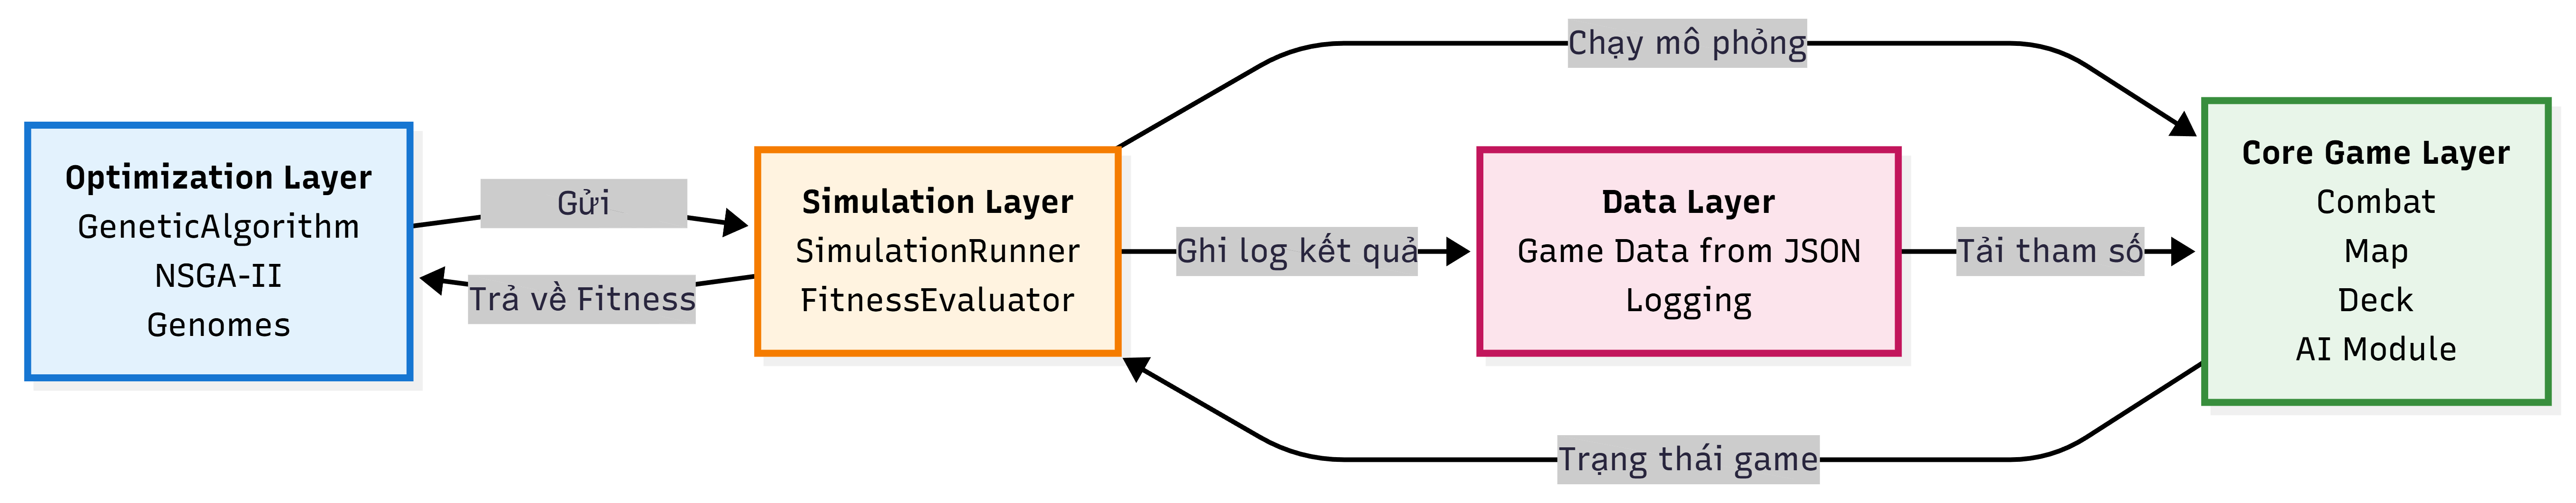
\includegraphics[width=0.9\textwidth]{SystemStructure.png}
    \caption{Kiến trúc tổng thể của hệ thống.}
    \label{fig:architecture}
\end{figure}

\section{Thiết kế chi tiết các module}

\subsection{Genome Representation}
Hai cách tiếp cận tối ưu hóa đòi hỏi hai cách biểu diễn genome khác nhau.

\subsubsection{BalanceGenome trong GA đơn mục tiêu}
Genome này biểu diễn trực tiếp từng tham số của game, tạo ra một không gian tìm kiếm lớn (~500 tham số). Nó bao gồm các dictionaries ánh xạ từ ID của đối tượng game đến hệ số nhân:
\begin{itemize}
    \item \texttt{CardActionScalars}: Hệ số nhân cho sát thương/giáp của từng hành động trên thẻ bài.
    \item \texttt{CardCostModifiers}: Mức thay đổi mana cost cho từng thẻ bài.
    \item \texttt{EnemyHealthScalars}: Hệ số nhân cho máu của từng loại kẻ địch.
    \item \texttt{EnemyActionValueScalars}: Hệ số nhân cho sát thương/giáp của từng hành động của kẻ địch.
\end{itemize}
Cách tiếp cận này cho phép điều chỉnh chi tiết nhưng dễ bị "curse of dimensionality".

\subsubsection{HierarchicalGenome trong NSGA-II đa mục tiêu}
Genome này gom nhóm các tham số theo một cấu trúc phân cấp, giảm không gian tìm kiếm xuống còn ~50 tham số. Các tham số được tổ chức theo các tầng:
\begin{itemize}
    \item \textbf{Global Multipliers:} Các hệ số nhân toàn cục cho sát thương, máu, giáp, giá vàng.
    \item \textbf{Progression Scaling:} Các hệ số điều chỉnh độ khó theo từng giai đoạn của game (Early/Mid/Late game).
    \item \textbf{Category Scaling:} Các hệ số nhân theo loại thẻ (Tấn công, Kỹ năng, Sức mạnh) và độ hiếm của thẻ/kẻ địch (1 đến 5 sao).
    \item \textbf{Room Distribution:} Các trọng số để điều chỉnh tần suất xuất hiện của các loại phòng (Quái, Tinh Anh, Sự kiện, Cửa hàng, Nghỉ ngơi).
\end{itemize}
Thiết kế này giúp thuật toán tìm kiếm hiệu quả hơn và đảm bảo các giải pháp có tính nhất quán về mặt thiết kế.

\begin{lstlisting}[language=C, caption={Ví dụ cách HierarchicalGenome tính toán scaled damage cho thẻ bài}, label={lst:hierarchical_scaling}]
public int GetScaledCardDamage(CardData card, int floor)
{
    // Bat dau voi global multiplier
    float scalar = GlobalDamageMultiplier;
    
    // Nhan voi category scalars (Attack/Skill/Power)
    scalar *= CardTypeScalars[card.Type];
    
    // Nhan voi rarity scalars (1-5 sao)
    scalar *= CardStarScalars[card.StarRating];
    
    // Nhan voi progression scaling (Early/Mid/Late game)
    scalar *= GetProgressionScalar(floor, ScalingType.Damage);
    
    // Ap dung override cho the cu the (neu co)
    if (CardDamageOverrides.TryGetValue(card.Id, out float ovr))
        scalar *= ovr;
    
    // Tinh toan gia tri cuoi cung
    var damageAction = card.Actions
        .FirstOrDefault(a => a.Type == ActionType.DealDamage);
    if (damageAction == null) return 0;
    
    return Math.Max(1, (int)Math.Round(damageAction.Value * scalar));
}
\end{lstlisting}

\subsection{AI Agent Design (HeuristicPlayerAI)}
AI agent được thiết kế với các heuristics dựa trên luật để mô phỏng một người chơi có trình độ trung bình. Logic ra quyết định của AI được chia thành các phần:
\begin{itemize}
    \item \textbf{Trong chiến đấu:}
        \begin{itemize}
            \item \textit{Ưu tiên sống sót:} Tính toán tổng sát thương sắp nhận và ưu tiên chơi các thẻ phòng thủ để chặn sát thương.
            \item \textit{Ưu tiên kết liễu:} Nếu có thể kết liễu kẻ địch trong lượt, AI sẽ ưu tiên các thẻ tấn công.
            \item \textit{Tối ưu hiệu quả:} Nếu không có nguy hiểm trước mắt, AI sẽ chọn chơi các thẻ tấn công hoặc kỹ năng dựa trên một hàm tính điểm, ưu tiên hiệu quả trên mỗi mana.
        \end{itemize}
    \item \textbf{Trên bản đồ:} AI chọn đường đi dựa trên điểm số của từng phòng, được tính toán dựa trên phần trăm máu hiện tại. Ví dụ, nó sẽ ưu tiên phòng Tinh Anh (Elite) khi máu cao để tìm phần thưởng tốt hơn, và ưu tiên phòng Nghỉ (Rest) khi máu thấp.
    \item \textbf{Lựa chọn phần thưởng:} AI ưu tiên các thẻ bài có độ hiếm cao hơn và cố gắng cân bằng giữa thẻ tấn công và phòng thủ trong bộ bài.
\end{itemize}

\subsection{Data Flow Diagram}
Hình \ref{fig:dataflow} minh họa luồng dữ liệu trong hệ thống, từ khi genome được tạo ra đến khi fitness được tính toán. Quá trình bao gồm: (1) Optimization Layer tạo genomes, (2) GenomeApplicator áp dụng genome vào GameData, (3) Simulation Runner chạy game với AI agent, (4) SimulationStats được thu thập, và (5) Fitness Evaluator tính toán fitness từ stats.

\begin{figure}[H]
    \centering
    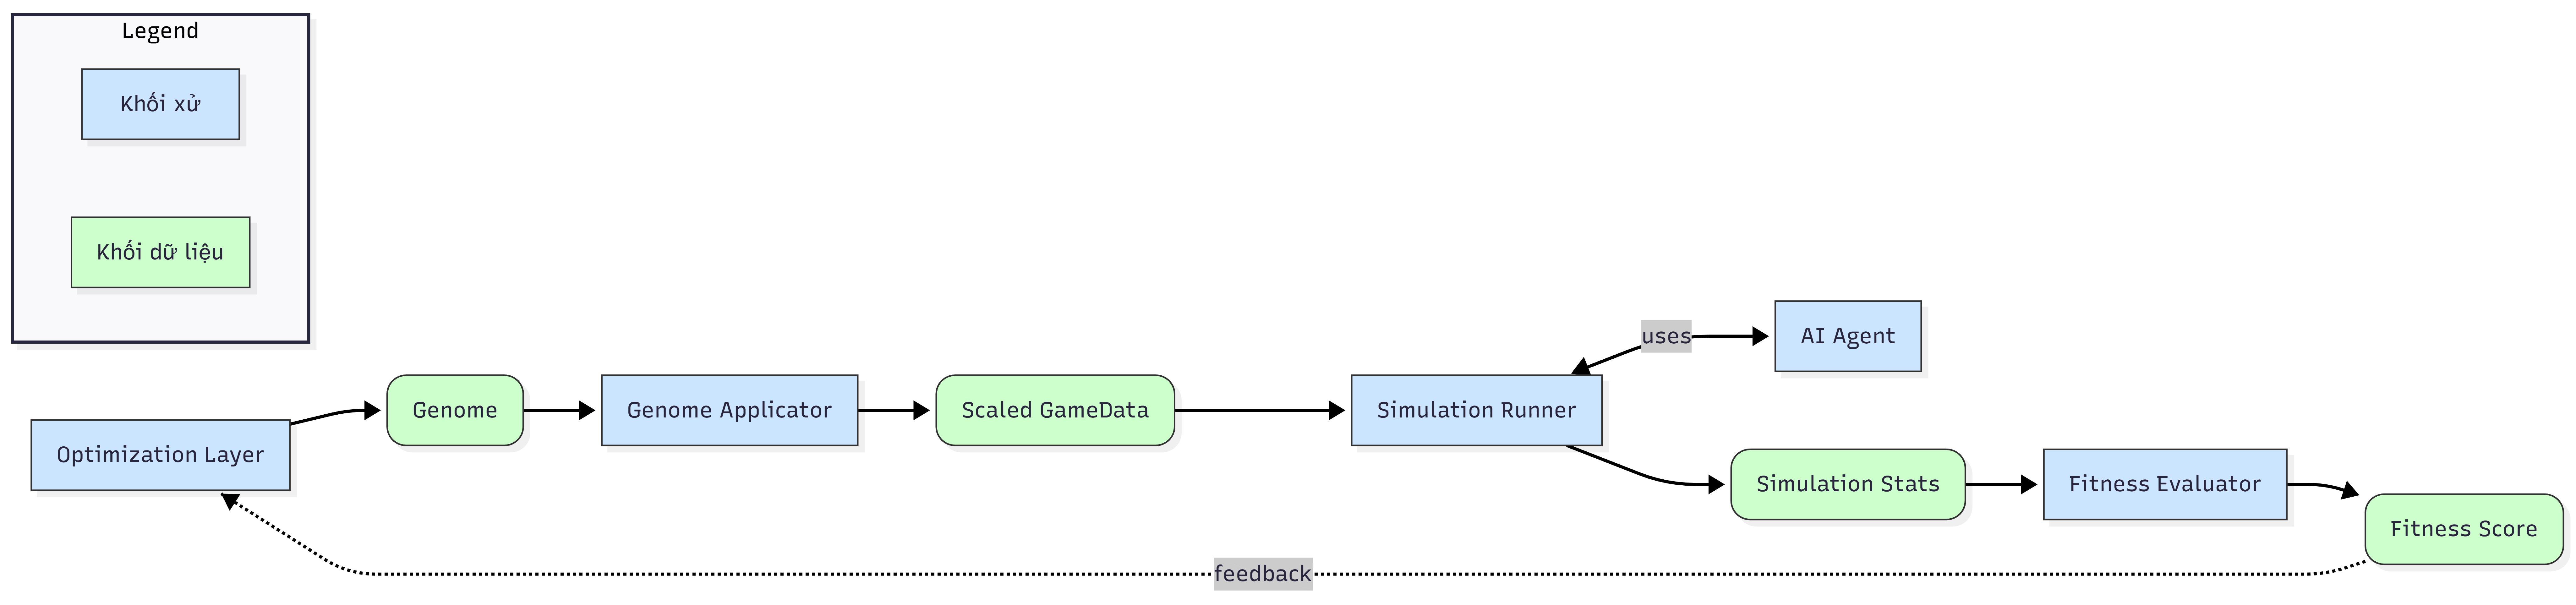
\includegraphics[width=0.9\textwidth]{dataflow.png}
    \caption{Sơ đồ luồng dữ liệu trong hệ thống}
    \label{fig:dataflow}
\end{figure}

\subsection{Combat Sequence Diagram}
Hình \ref{fig:combat_sequence} mô tả trình tự tương tác giữa các thành phần trong một lượt chiến đấu điển hình. Mỗi lượt bắt đầu với việc rút bài, sau đó AI quyết định chơi thẻ nào, CombatManager xử lý actions, và kẻ địch phản ứng lại. Quá trình lặp lại cho đến khi một bên thua.

\begin{figure}[H]
    \centering
    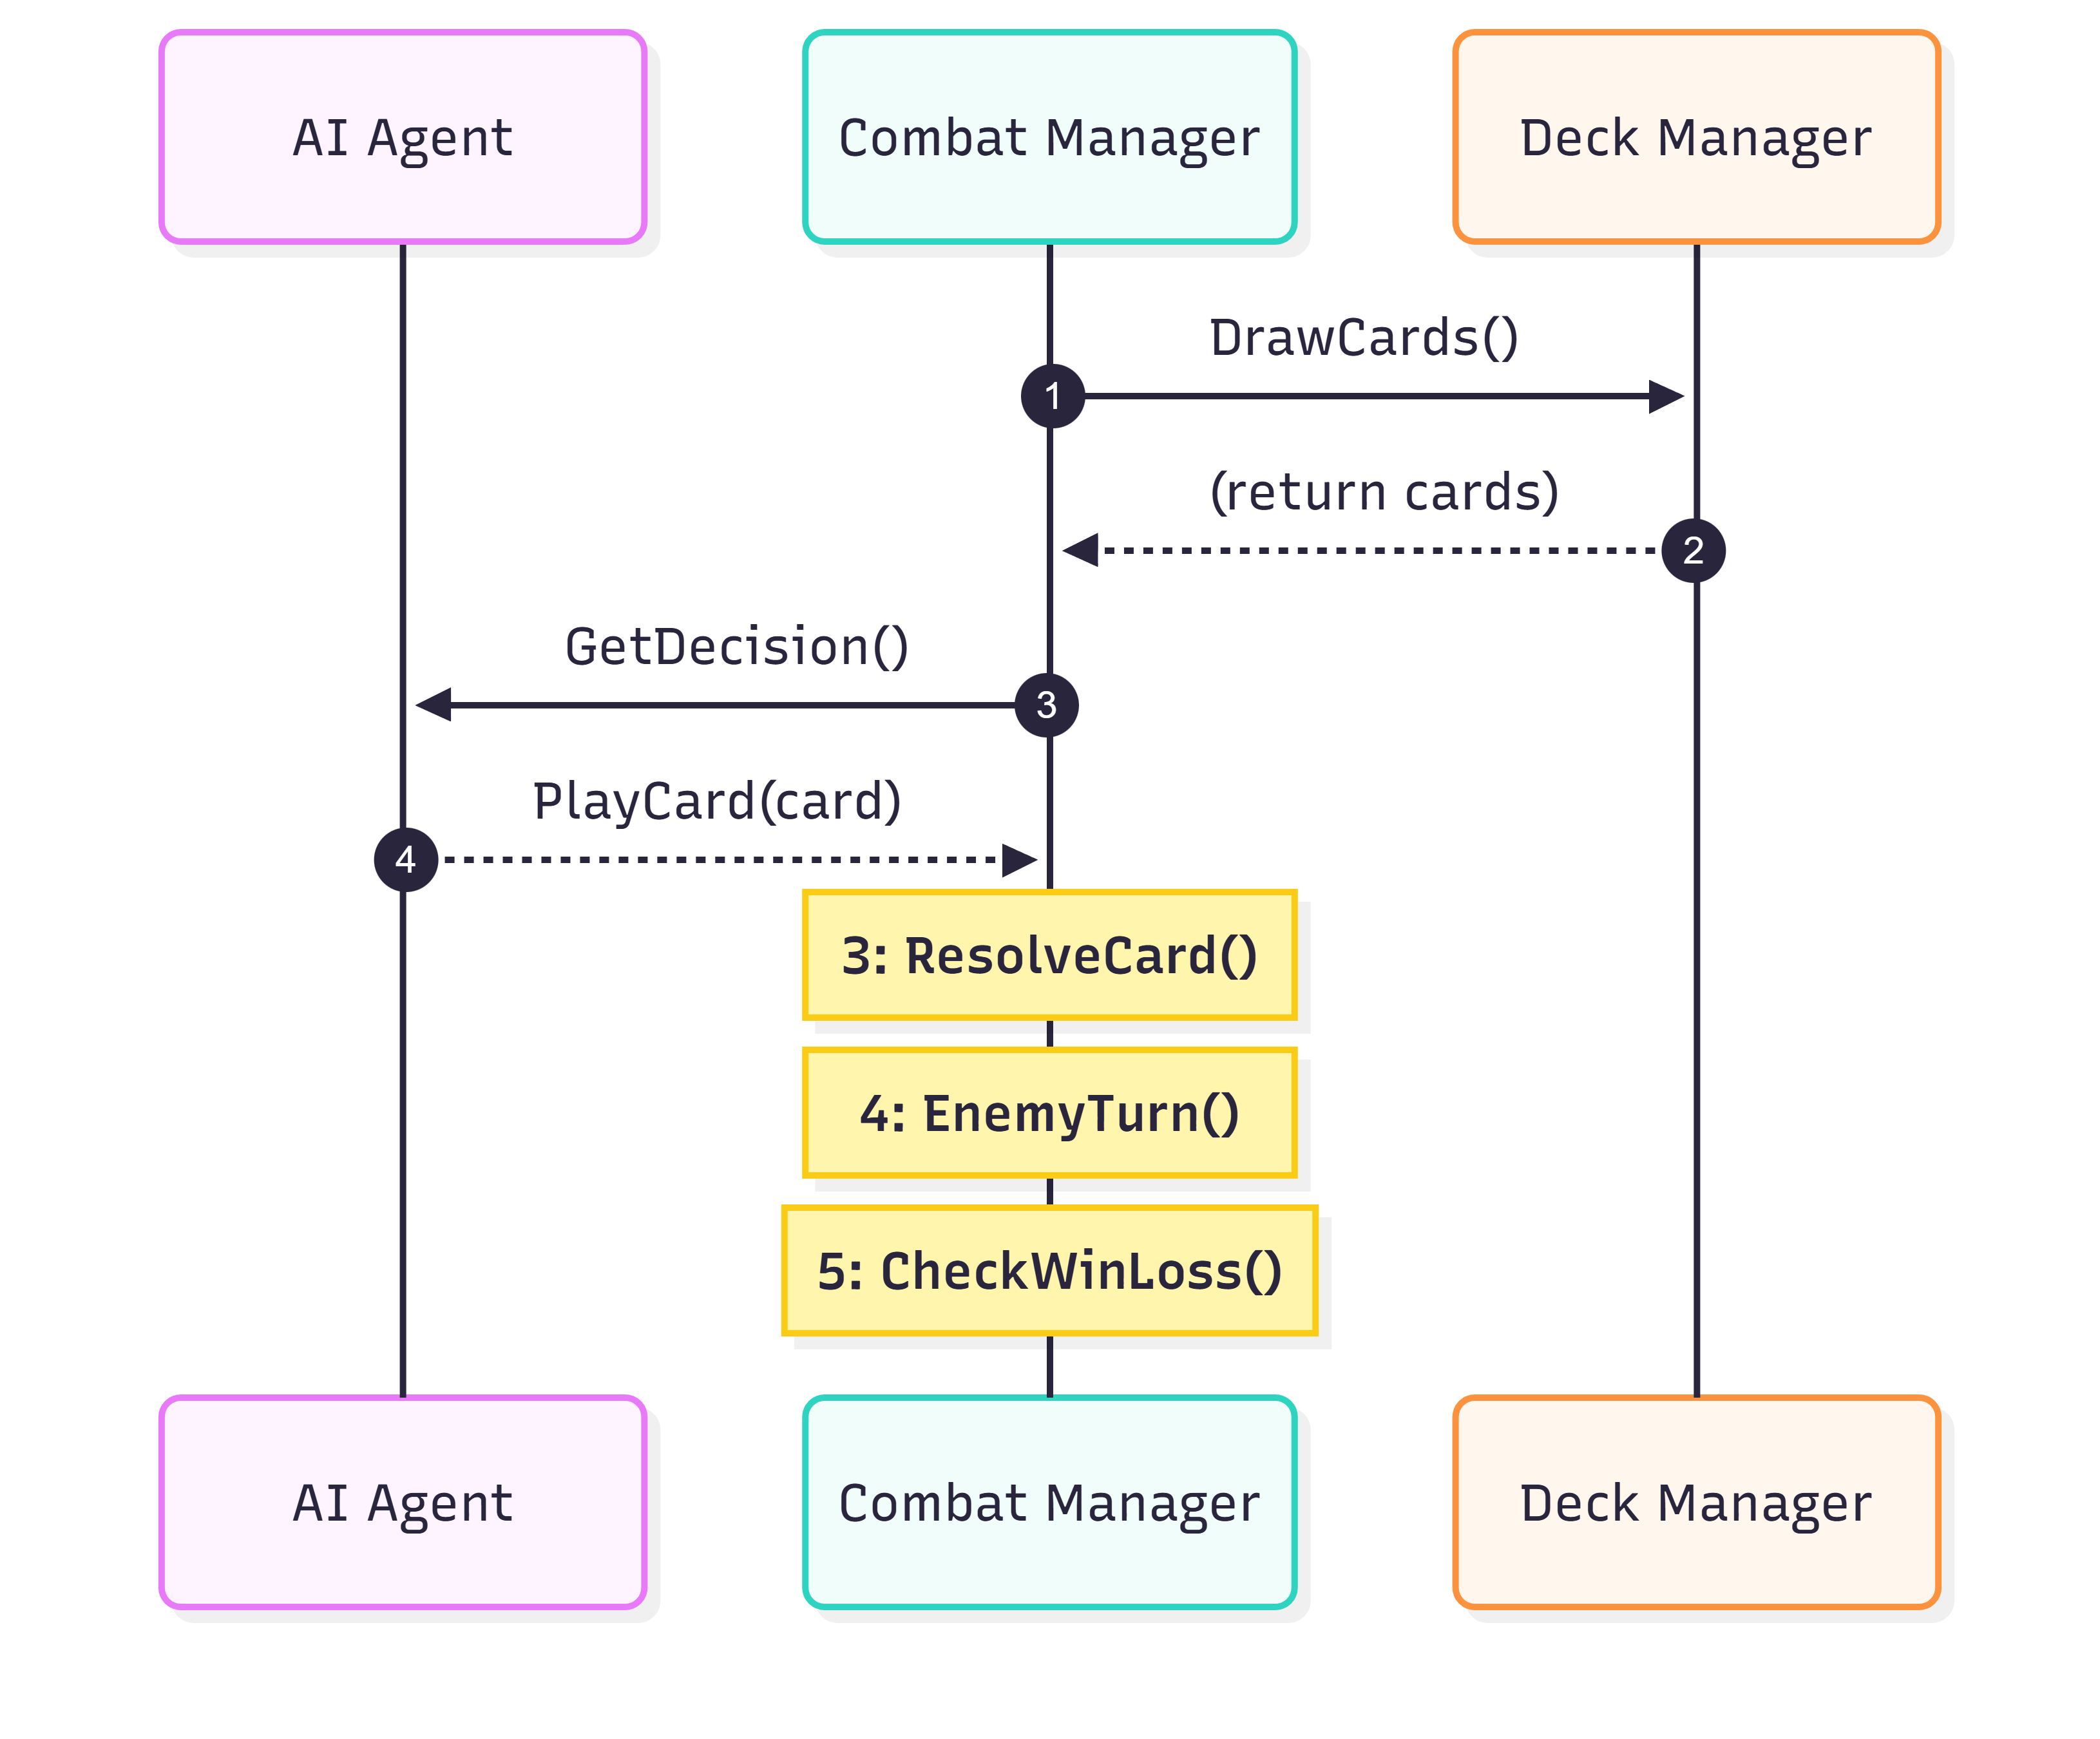
\includegraphics[width=0.6\textwidth]{combat_sequence.png}
    \caption{Sequence diagram của một lượt chiến đấu}
    \label{fig:combat_sequence}
\end{figure}

\subsection{Class Diagram}
Hình \ref{fig:class_diagram} thể hiện các class chính và mối quan hệ giữa chúng. Các module được tổ chức thành các tầng rõ ràng, với Core Game Layer (GameController, CombatManager, DeckManager), AI Layer (HeuristicPlayerAI), và Optimization Layer (GeneticAlgorithm, NSGA2Optimizer).

\begin{figure}[H]
    \centering
    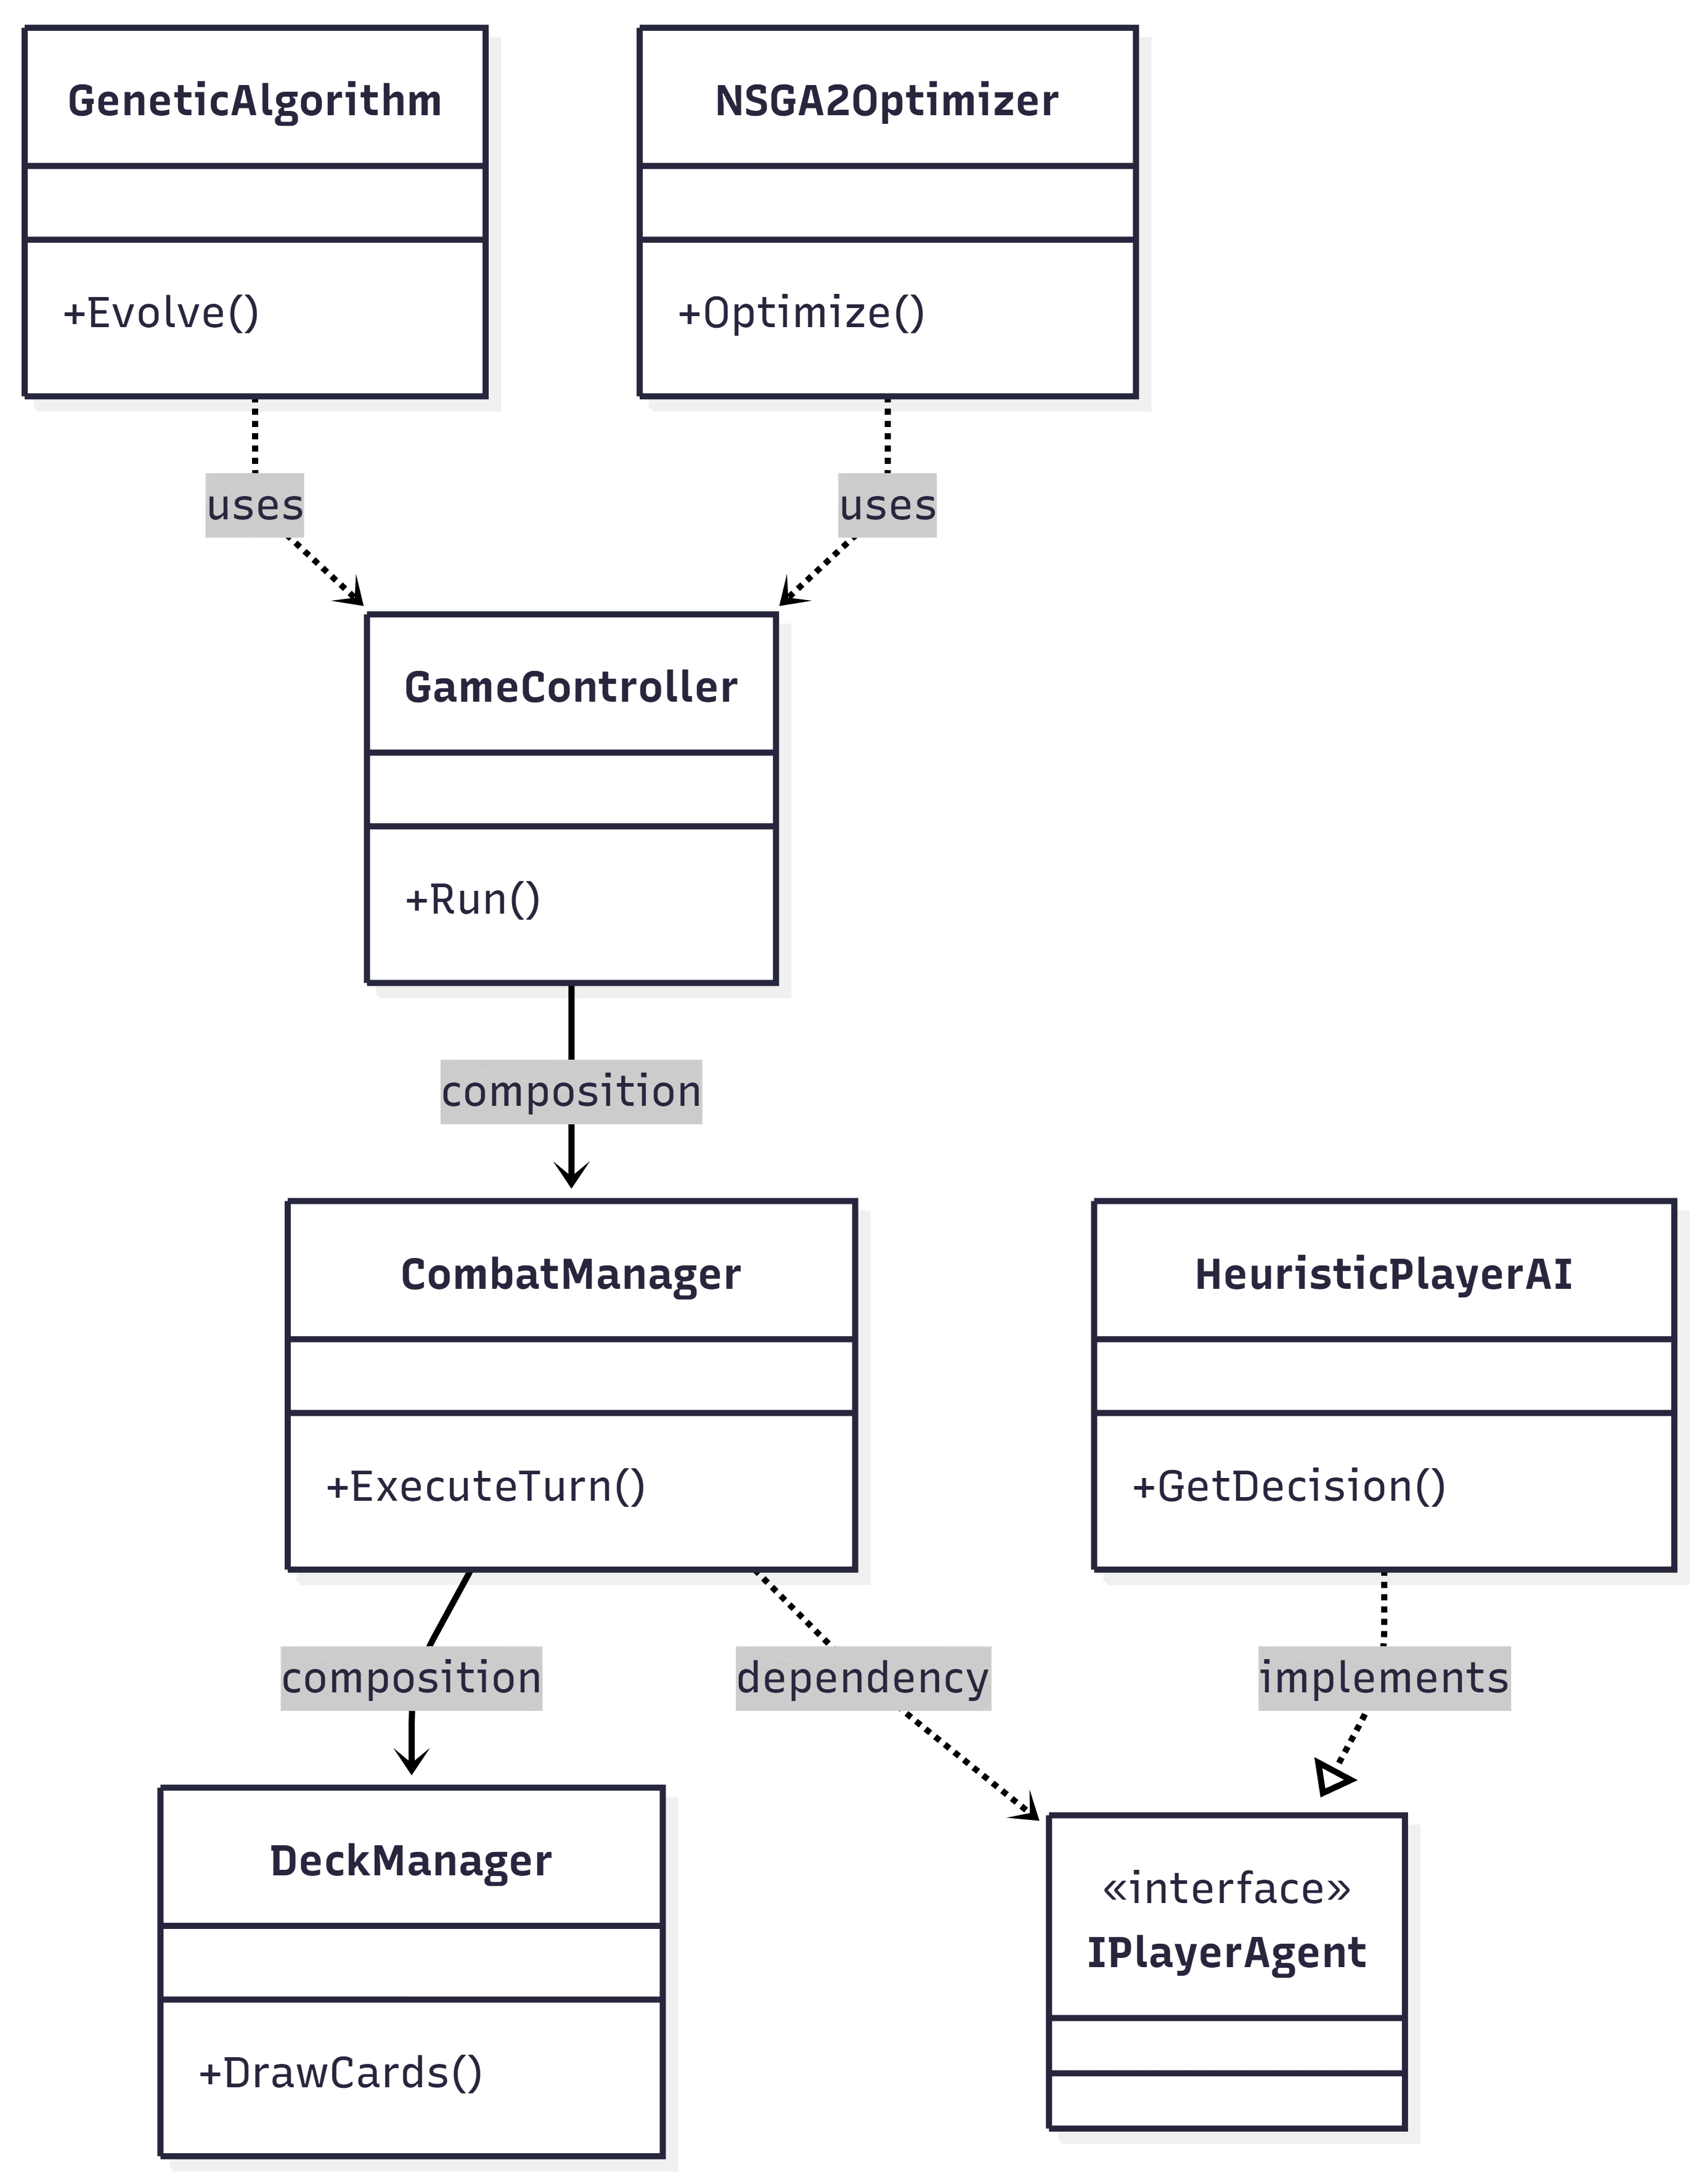
\includegraphics[width=0.6\textwidth]{class_diagram.png}
    \caption{Class diagram của các module chính}
    \label{fig:class_diagram}
\end{figure}

\subsection{Fitness Evaluation}
Đối với phương pháp structure-aware sử dụng NSGA-II, hệ thống tối ưu hóa đồng thời 3 mục tiêu:
\begin{enumerate}
    \item \textbf{Balance Score:} Đo lường độ cân bằng của game bằng cách so sánh các chỉ số thực tế (tỷ lệ thắng, HP khi thắng, tầng khi thua) với các giá trị mục tiêu (target). Balance Score được tính bằng:
    \begin{equation}
    f_{balance} = \sum_{i} w_i \cdot \left| \frac{\text{actual}_i - \text{target}_i}{\text{target}_i} \right|
    \end{equation}
    trong đó $w_i$ là trọng số quan trọng của metric thứ $i$.
    
    \item \textbf{Engagement Score:} Đánh giá sự hấp dẫn và đa dạng chiến thuật, dựa trên số lượng thẻ bài "khả dụng" (Viable Cards) và sự đa dạng trong các lối xây dựng bộ bài (Build Variety):
    \begin{equation}
    f_{engagement} = \alpha \cdot \frac{|\text{ViableCards}|}{|\text{TotalCards}|} + \beta \cdot \text{BuildDiversity}
    \end{equation}
    với $\alpha, \beta$ là các trọng số cân bằng. Càng nhiều thẻ bài khả dụng và càng đa dạng lối chơi thì Engagement Score càng cao.
    
    \item \textbf{Coherence Score:} Đo lường tính nhất quán trong thiết kế. Điểm số được tính bằng cách lấy 1 trừ đi tổng hình phạt (penalty):
    \begin{equation}
    f_{coherence} = 1 - \left( \text{TrapCardPenalty} + \lambda \cdot \sum_{j} (\text{scalar}_j - 1)^2 \right)
    \end{equation}
    trong đó TrapCardPenalty phạt nặng các "thẻ bài rác" (Trap Cards - thẻ được chọn nhưng có tỷ lệ thắng thấp), và $\lambda$ kiểm soát mức độ phạt cho các tham số xa giá trị chuẩn. Khi không có trap cards và các scalars gần 1.0, Coherence Score đạt giá trị tối đa.
\end{enumerate}
Đối với phương pháp GA truyền thống, ba chỉ số trên được kết hợp thành một hàm fitness duy nhất:
\begin{equation}
F_{total} = w_1 \cdot f_{balance} + w_2 \cdot f_{engagement} + w_3 \cdot f_{coherence}
\end{equation}
\newpage
\clearpage
\phantomsection
\chapter{CÀI ĐẶT VÀ TRIỂN KHAI}

\section{Môi trường phát triển}

Hệ thống được phát triển bằng ngôn ngữ C\# trên nền tảng .NET 9.0, đảm bảo hiệu năng cao và khả năng chạy đa nền tảng.
\begin{itemize}
    \item \textbf{Ngôn ngữ lập trình:} C\# 13.0
    \item \textbf{Framework:} .NET 9.0
    \item \textbf{IDE:} Visual Studio Code 1.107.0
    \item \textbf{Quản lý phiên bản:} Git và GitHub
    \item \textbf{Định dạng dữ liệu:} JSON được sử dụng để lưu trữ toàn bộ dữ liệu game (thẻ bài, kẻ địch, di vật) và cấu hình thuật toán.
\end{itemize}

\subsection{Cấu trúc dự án}
Dự án được tổ chức theo cấu trúc module rõ ràng để dễ dàng quản lý và mở rộng.
\begin{lstlisting}[language=bash, caption={Cấu trúc thư mục dự án}]
RoguelikeDeckBuilder/
|-- src/
|   |-- Roguelike/
|   |   |-- Core/           # Core game engine
|   |   |   |-- AI/
|   |   |   |-- Combat/
|   |   |   |-- Data/
|   |   |   |-- Map/
|   |   |-- Optimization/   # Optimization modules
|   |   |   |-- GASingleObjective/
|   |   |   |-- NSGA2MultiObjective/
|   |   |-- Program.cs      # Entry point
|   |   |-- GameData.json   # Game data
\end{lstlisting}

\section{Triển khai các module cốt lõi}

\subsection{Core Game Layer}
Tầng lõi của game được hiện thực hóa qua các lớp C\# chính:
\begin{itemize}
    \item \texttt{GameController.cs:} Lớp điều phối chính, xử lý các luồng trạng thái của game (bản đồ, chiến đấu, sự kiện, phần thưởng).
    \item \texttt{CombatManager.cs:} Quản lý logic chiến đấu theo lượt, bao gồm việc chơi bài, hành động của kẻ địch, áp dụng hiệu ứng và kiểm tra điều kiện thắng/thua.
    \item \texttt{DeckManager.cs:} Quản lý các chồng bài (rút, bỏ, trên tay) và các thao tác như xào bài, rút bài.
    \item \texttt{MapGenerator.cs:} Sử dụng thuật toán sinh ngẫu nhiên có ràng buộc để tạo ra bản đồ các phòng hợp lệ cho mỗi lượt chơi.
\end{itemize}

\subsection{AI Agent}
Lớp \texttt{HeuristicPlayerAI.cs} hiện thực hóa giao diện \texttt{IPlayerAgent}, cung cấp logic cho các quyết định của AI tại mỗi trạng thái của game. Các hàm tính điểm được sử dụng để đánh giá nước đi tốt nhất trong chiến đấu và trên bản đồ.

\begin{lstlisting}[language=C, caption={Logic ra quyết định trong chiến đấu của AI agent}, label={lst:ai_combat_decision}]
public CombatDecision GetCombatDecision(GameRun run)
{
    var hero = run.TheHero;
    var enemies = run.CurrentCombat.Enemies
        .Where(e => e.CurrentHealth > 0).ToList();
    
    // Tinh toan sat thuong sap nhan
    int totalIncomingDamage = CalculateIncomingDamage(run, enemies);
    int neededBlock = Math.Max(0, totalIncomingDamage - hero.Block);

    // UU TIEN 1: SINH TON - Choi the phong thu neu can
    if (neededBlock > 0)
    {
        var defensiveMove = FindBestDefensiveMove(
            run, hero, enemies, neededBlock);
        if (defensiveMove.HasValue)
            return defensiveMove.Value;
    }

    // UU TIEN 2: KET LIEU - Tim nuoc danh ket lieu ke dich
    var lethalMove = FindLethalMove(run, hero, enemies);
    if (lethalMove.HasValue)
        return lethalMove.Value;

    // UU TIEN 3: NUOC DI TOT NHAT - Choi the co diem cao nhat
    return GetBestGeneralMove(run, hero, enemies);
}
\end{lstlisting}

\section{Triển khai các module tối ưu hóa}
\subsection{GA đơn mục tiêu}
\begin{itemize}
    \item \texttt{GeneticAlgorithm.cs:} Lớp chính điều khiển vòng lặp tiến hóa, bao gồm chọn lọc, lai ghép và đột biến.
    \item \texttt{BalanceGenome.cs:} Biểu diễn bộ gen dưới dạng các `Dictionary` chứa các hệ số nhân cho từng tham số game.
    \item \texttt{FitnessEvaluator.cs:} Tính toán một giá trị fitness duy nhất từ kết quả của nhiều lượt mô phỏng.
\end{itemize}
\subsection{NSGA-II đa mục tiêu}
\begin{itemize}
    \item \texttt{ImprovedGeneticAlgorithm.cs:} Lớp điều khiển chính, sử dụng \texttt{NSGA2Optimizer}.
    \item \texttt{NSGA2Optimizer.cs:} Hiện thực hóa các thuật toán cốt lõi của NSGA-II:
        \begin{itemize}
            \item \texttt{FastNonDominatedSort}: Phân loại quần thể thành các Pareto front.
            \item \texttt{CalculateCrowdingDistance}: Tính toán khoảng cách đám đông để duy trì sự đa dạng.
            \item Sử dụng các toán tử lai ghép (Simulated Binary Crossover - SBX) và đột biến (Polynomial Mutation) phù hợp cho các giá trị thực.
        \end{itemize}
    \item \texttt{HierarchicalGenome.cs:} Biểu diễn bộ gen phân cấp với các thuộc tính cho từng nhóm tham số.
    \item \texttt{MultiObjectiveFitness.cs:} Tính toán 3 giá trị fitness riêng biệt (Balance, Engagement, Coherence).
\end{itemize}
\begin{lstlisting}[language=C, caption={Thuật toán Fast Non-Dominated Sort của NSGA-II}, label={lst:nsga2_sort}]
public List<List<Individual>> FastNonDominatedSort(
    List<Individual> population)
{
    var fronts = new List<List<Individual>>();
    var dominationCount = new Dictionary<Individual, int>();
    var dominatedSolutions = new Dictionary<Individual, List<Individual>>();
    
    // Tim cac moi quan he domination
    var firstFront = new List<Individual>();
    foreach (var p in population)
    {
        foreach (var q in population)
        {
            if (p == q) continue;
            if (p.Fitness.Dominates(q.Fitness))
                dominatedSolutions[p].Add(q);
            else if (q.Fitness.Dominates(p.Fitness))
                dominationCount[p]++;
        }
        
        // Neu khong bi dominated boi ai => Front 1
        if (dominationCount[p] == 0)
        {
            p.Fitness.Rank = 1;
            firstFront.Add(p);
        }
    }
    fronts.Add(firstFront);
    
    // Xay dung cac front tiep theo
    int currentRank = 1;
    while (fronts[currentRank - 1].Any())
    {
        var nextFront = new List<Individual>();
        foreach (var p in fronts[currentRank - 1])
        {
            foreach (var q in dominatedSolutions[p])
            {
                dominationCount[q]--;
                if (dominationCount[q] == 0)
                {
                    q.Fitness.Rank = currentRank + 1;
                    nextFront.Add(q);
                }
            }
        }
        if (nextFront.Any())
        {
            fronts.Add(nextFront);
            currentRank++;
        }
        else break;
    }
    return fronts;
}
\end{lstlisting}

\begin{lstlisting}[language=C, caption={Tính toán Crowding Distance để duy trì diversity}, label={lst:crowding_distance}]
public void CalculateCrowdingDistance(List<Individual> front)
{
    int n = front.Count;
    if (n == 0) return;
    
    // Khoi tao distance = 0
    foreach (var ind in front)
        ind.Fitness.CrowdingDistance = 0;
    
    // Voi moi objective (Balance, Engagement, Coherence)
    var objectives = new Func<MultiObjectiveFitness, float>[]
    {
        f => f.BalanceScore,
        f => f.EngagementScore,
        f => f.CoherenceScore
    };
    
    foreach (var objective in objectives)
    {
        // Sap xep theo objective nay
        var sorted = front.OrderBy(ind => objective(ind.Fitness))
            .ToList();
        
        // Cac giai phap o bien duoc gan distance vo cung
        sorted[0].Fitness.CrowdingDistance = float.MaxValue;
        sorted[n-1].Fitness.CrowdingDistance = float.MaxValue;
        
        float range = objective(sorted[n-1].Fitness) 
                    - objective(sorted[0].Fitness);
        if (range < 1e-6) continue;
        
        // Tinh crowding distance cho cac giai phap giua
        for (int i = 1; i < n - 1; i++)
        {
            float distance = (objective(sorted[i+1].Fitness) - 
                             objective(sorted[i-1].Fitness)) / range;
            sorted[i].Fitness.CrowdingDistance += distance;
        }
    }
}
\end{lstlisting}

\begin{lstlisting}[language=C, caption={Hàm kiểm tra Pareto dominance giữa hai giải pháp}, label={lst:dominates}]
public bool Dominates(MultiObjectiveFitness other)
{
    // Constraint-domination: giai phap kha thiluon tot hon khong kha thi
    if (this.IsFeasible && !other.IsFeasible) return true;
    if (!this.IsFeasible && other.IsFeasible) return false;
    
    // Ca hai khong kha thi: so sanh so luong rang buoc vi pham
    if (!this.IsFeasible && !other.IsFeasible)
        return this.ConstraintViolations < other.ConstraintViolations;
    
    // Ca hai kha thi: Pareto domination chuan
    bool atLeastOneBetter = false;
    
    // Phai >= voi tat ca cac objective
    if (BalanceScore < other.BalanceScore) return false;
    if (EngagementScore < other.EngagementScore) return false;
    if (CoherenceScore < other.CoherenceScore) return false;
    
    // Va phai tot hon strict o it nhat 1 objective
    if (BalanceScore > other.BalanceScore) atLeastOneBetter = true;
    if (EngagementScore > other.EngagementScore) atLeastOneBetter = true;
    if (CoherenceScore > other.CoherenceScore) atLeastOneBetter = true;
    
    return atLeastOneBetter;
}
\end{lstlisting}

\begin{lstlisting}[language=C, caption={Tính toán Balance Score từ các metrics gameplay}, label={lst:balance_score}]
private float CalculateBalanceScore(List<SimulationStats> results)
{
    // Tinh cac metrics thuc te
    float actualWinRate = (float)results.Count(r => r.IsVictory) / results.Count;
    
    var victories = results.Where(r => r.IsVictory).ToList();
    float actualVictoryHp = victories.Any() 
        ? victories.Average(r => (float)r.FinalHeroHP / r.FinalHeroMaxHP)
        : 0f;
    
    var deaths = results.Where(r => !r.IsVictory).ToList();
    float actualFloorOnDeath = deaths.Any()
        ? deaths.Average(r => r.FinalFloor)
        : 0f;
    
    // Cac gia tri muc tieu
    const float targetWinRate = 0.45f;
    const float targetVictoryHp = 0.30f;
    const float targetFloorOnDeath = 10f;
    
    // Tinh chenh lech chuan hoa
    float wrDeviation = Math.Abs(actualWinRate - targetWinRate) / targetWinRate;
    float hpDeviation = Math.Abs(actualVictoryHp - targetVictoryHp) / targetVictoryHp;
    float floorDeviation = Math.Abs(actualFloorOnDeath - targetFloorOnDeath) 
                          / targetFloorOnDeath;
    
    // Ket hop voi trong so
    float totalDeviation = 
        0.50f * wrDeviation +      // Win rate quan trong nhat
        0.30f * hpDeviation +      // Victory HP
        0.20f * floorDeviation;    // Floor on death
    
    // Chuyen thanh diem (1.0 = hoan hao, 0.0 = sai lech lon)
    return Math.Max(0f, 1.0f - totalDeviation);
}
\end{lstlisting}

\section{Thách thức và giải pháp}
\begin{itemize}
    \item \textbf{Tối ưu hóa hiệu năng:} Việc chạy hàng trăm nghìn lượt mô phỏng đòi hỏi hiệu năng cao. Giải pháp là sử dụng \texttt{Parallel.ForEach} của .NET để chạy các mô phỏng song song, tận dụng tối đa các lõi CPU.
    \item \textbf{Không gian tìm kiếm lớn:} Với phương pháp GA đơn mục tiêu, không gian ~500 chiều là một thách thức lớn. Giải pháp NSGA-II đa mục tiêu với \texttt{HierarchicalGenome} đã giảm không gian này xuống còn ~50 chiều, giúp thuật toán hội tụ nhanh và hiệu quả hơn.
    \item \textbf{Đảm bảo tính nhất quán:} Các thay đổi ngẫu nhiên của GA có thể tạo ra các tham số vô lý. Giải pháp là áp dụng các ràng buộc trong quá trình đột biến và lai ghép, đồng thời thiết kế \texttt{HierarchicalGenome} để các thay đổi mang tính tương đối thay vì tuyệt đối.
\end{itemize}
\newpage
\clearpage
\phantomsection
\chapter{THỰC NGHIỆM VÀ ĐÁNH GIÁ}

\section{Thiết lập thực nghiệm}
Thực nghiệm được tiến hành để so sánh hiệu quả của hai phương pháp: GA đơn mục tiêu và NSGA-II đa mục tiêu.

\subsection{Cấu hình hệ thống}
\begin{itemize}
    \item \textbf{CPU:} AMD Ryzen 7 6800H với Radeon Graphics, 3201Mhz, 8 Cores, 16 Threads
    \item \textbf{RAM:} 24 GB DDR5 4800MHz
    \item \textbf{Hệ điều hành:} Microsoft Windows 11
    \item \textbf{Nền tảng:} .NET 9.0
\end{itemize}

\subsection{Tham số thuật toán}
Bảng \ref{tab:algorithm_params} chi tiết các tham số cấu hình cho cả hai phương pháp tối ưu hóa.

\begin{table}[H]
    \centering
    \caption{So sánh chi tiết các tham số thuật toán.}
    \label{tab:algorithm_params}
    \begin{tabular}{l c c}
        \toprule
        \textbf{Tham số} & \textbf{GA đơn mục tiêu} & \textbf{NSGA-II đa mục tiêu} \\
        \midrule
        \multicolumn{3}{c}{\textit{Tham số chung}} \\
        \midrule
        Population Size & 100 & 100 \\
        Number of Generations & 30 & 30 \\
        Simulations per Genome & 200 (cố định) & 200 (adaptive) \\
        \addlinespace
        \multicolumn{3}{c}{\textit{Không gian tìm kiếm}} \\
        \midrule
        Genome Representation & BalanceGenome & HierarchicalGenome \\
        Số lượng tham số & \textasciitilde 500 & \textasciitilde 50 \\
        \addlinespace
        \multicolumn{3}{c}{\textit{Toán tử di truyền}} \\
        \midrule
        Selection Method & Tournament (k=3) & Binary Tournament \\
        Crossover Type & Uniform Crossover & Simulated Binary (SBX) \\
        Crossover Rate & 0.8 & 0.9 \\
        Mutation Type & Gaussian & Polynomial \\
        Mutation Rate & 0.02 (2\%) & 0.05 (5\%) \\
        Mutation Strength ($\sigma$) & 0.1 & Adaptive \\
        \addlinespace
        \multicolumn{3}{c}{\textit{Chiến lược tiến hóa}} \\
        \midrule
        Elitism & Top 10\% & All Pareto Front \\
        Diversity Mechanism & Random immigrants & Crowding Distance \\
        Fitness Function & Weighted sum & Multi-objective \\
        \addlinespace
        \multicolumn{3}{c}{\textit{Tối ưu hóa}} \\
        \midrule
        Parallelization & Yes (8 cores) & Yes (8 cores) \\
        Adaptive Evaluation & No & Yes (50-200 sims) \\
        Early Stopping & No & Convergence-based \\
        \bottomrule
    \end{tabular}
\end{table}

Các tham số được điều chỉnh dựa trên đặc trưng của từng phương pháp. NSGA-II sử dụng mutation rate cao hơn (5\% so với 2\%) để duy trì đa dạng trên Pareto front, trong khi GA đơn mục tiêu dùng elitism đơn giản (top 10\%) thay vì bảo toàn toàn bộ Pareto front.

\subsection{Các chỉ số mục tiêu (Target Metrics)}
\begin{itemize}
    \item \textbf{Target Win Rate:} 45\% (Thách thức nhưng có thể đạt được).
    \item \textbf{Target Victory HP:} 30\% HP còn lại (Các trận thắng không quá dễ dàng).
    \item \textbf{Target Floor on Death:} 10 (Người chơi có trải nghiệm đủ sâu trước khi thua).
\end{itemize}

\section{Kết quả thực nghiệm}
\subsection{Phương pháp 1: GA đơn mục tiêu}
Sau 30 thế hệ, phương pháp GA truyền thống đã cho thấy sự cải thiện đáng kể trong việc tối ưu hóa hàm fitness tổng hợp.
\begin{itemize}
    \item \textbf{Overall Fitness:} Tăng từ \textbf{1.45} lên \textbf{32.66} (+2150\%), cho thấy thuật toán đã tìm được các giải pháp tốt hơn đáng kể.
    \item \textbf{Win Rate:} Tăng từ \textbf{36.0\%} lên \textbf{38.3\%} (+6.4\%). Mặc dù chưa đạt mục tiêu 45\%, xu hướng cải thiện cho thấy game đang tiến gần hơn đến độ cân bằng mong muốn.
    \item \textbf{Victory HP:} Cải thiện từ \textbf{59.95\%} xuống còn \textbf{40.87\%} HP còn lại khi thắng, tiến gần hơn đến mục tiêu 30\%, cho thấy các trận thắng đã trở nên "sát sao" và kịch tính hơn.
    \item \textbf{Floor on Death:} Giảm từ \textbf{12.22} xuống \textbf{10.57}, gần đạt mục tiêu 10, cho thấy độ khó đã được điều chỉnh hợp lý hơn.
    \item \textbf{Thời gian chạy:} \textbf{73 phút} cho 30 thế hệ.
\end{itemize}
Tuy nhiên, phương pháp này không cải thiện được sự đa dạng chiến thuật, số lượng thẻ bài khả dụng (Viable Cards) vẫn giữ nguyên ở mức 12, và Build Variety chỉ tăng từ 0.616 lên 0.680.

\subsection{Phương pháp 2: NSGA-II đa mục tiêu}
Phương pháp NSGA-II với bộ gen phân cấp không chỉ tối ưu hóa các chỉ số cân bằng mà còn cải thiện đáng kể trải nghiệm chơi. Kết quả được lấy từ giải pháp "thỏa hiệp tốt nhất" trên Pareto front cuối cùng.

\begin{lstlisting}[language=C, caption={Đánh giá Pareto domination và tính Balance Score}, label={lst:fitness_eval}]
// Kiem tra xem giai phap nay co dominate giai phap khac khong
public bool Dominates(MultiObjectiveFitness other)
{
    // Constraint-domination: feasible luon dominate infeasible
    if (this.IsFeasible && !other.IsFeasible) return true;
    if (!this.IsFeasible && other.IsFeasible) return false;
    
    // Ca hai feasible: Pareto domination binh thuong
    bool atLeastOneBetter = false;
    
    // Phai >= o tat ca cac objectives
    if (BalanceScore < other.BalanceScore) return false;
    if (EngagementScore < other.EngagementScore) return false;
    if (CoherenceScore < other.CoherenceScore) return false;
    
    // Va tot hon thuc su o it nhat mot objective
    if (BalanceScore > other.BalanceScore) atLeastOneBetter = true;
    if (EngagementScore > other.EngagementScore) atLeastOneBetter = true;
    if (CoherenceScore > other.CoherenceScore) atLeastOneBetter = true;
    
    return atLeastOneBetter;
}

// Tinh Balance Score su dung Gaussian-like scoring
private float CalculateBalanceScore(MultiObjectiveFitness f)
{
    // Do sai lech so voi target metrics
    float winRateDiff = Math.Abs(f.WinRate - TargetWinRate);
    float victoryHpDiff = Math.Abs(f.VictoryHp - TargetVictoryHp);
    float floorDeathDiff = Math.Abs(f.AvgFloorOnDeath - TargetAvgFloorOnDeath);
    
    // Gaussian scoring: 1.0 = perfect, 0.0 = rat xa target
    const float WIN_RATE_SENSITIVITY = 10.0f;
    const float VICTORY_HP_SENSITIVITY = 8.0f;
    const float FLOOR_DEATH_SENSITIVITY = 0.05f;
    
    float wrScore = (float)Math.Exp(
        -WIN_RATE_SENSITIVITY * winRateDiff * winRateDiff);
    float hpScore = (float)Math.Exp(
        -VICTORY_HP_SENSITIVITY * victoryHpDiff * victoryHpDiff);
    float floorScore = (float)Math.Exp(
        -FLOOR_DEATH_SENSITIVITY * floorDeathDiff * floorDeathDiff);
    
    return (wrScore + hpScore + floorScore) / 3.0f;
}
\end{lstlisting}

Balance Score được tính dựa trên hàm Gaussian để đánh giá mức độ gần với các chỉ số mục tiêu. Công thức toán học tổng quát là:
\begin{equation}
f_{balance} = \frac{1}{3}\left(\exp(-\alpha_{wr} \cdot \Delta_{wr}^2) + \exp(-\alpha_{hp} \cdot \Delta_{hp}^2) + \exp(-\alpha_{fd} \cdot \Delta_{fd}^2)\right)
\end{equation}
trong đó:
\begin{itemize}
    \item $\Delta_{wr} = |\text{WinRate} - \text{TargetWinRate}|$ là độ lệch tỷ lệ thắng
    \item $\Delta_{hp} = |\text{VictoryHP} - \text{TargetVictoryHP}|$ là độ lệch HP khi thắng
    \item $\Delta_{fd} = |\text{FloorOnDeath} - \text{TargetFloorOnDeath}|$ là độ lệch tầng khi thua
    \item $\alpha_{wr} = 10.0$, $\alpha_{hp} = 8.0$, $\alpha_{fd} = 0.05$ là các hệ số độ nhạy (sensitivity)
\end{itemize}
Hàm Gaussian này cho điểm 1.0 khi đạt chính xác mục tiêu và giảm dần về 0 khi càng xa mục tiêu, tạo gradient mượt mà giúp thuật toán tối ưu hiệu quả.

\begin{itemize}
    \item \textbf{Balance Score:} Tăng mạnh từ \textbf{0.754} lên \textbf{0.960} (+27.3\%), cho thấy game đã đạt được độ cân bằng cao về Win Rate, Victory HP và Floor on Death.
    \item \textbf{Engagement Score:} Cải thiện từ \textbf{0.655} lên \textbf{0.900} (+37.4\%). Đây là ưu điểm vượt trội, cho thấy sự đa dạng và hấp dẫn của game được cải thiện rõ rệt.
    \item \textbf{Coherence Score:} Tăng từ \textbf{0.853} lên \textbf{1.000} (+17.2\%), đảm bảo không có "thẻ bài rác" nào được tạo ra và tất cả các thẻ đều có ý nghĩa chiến thuật.
    \item \textbf{Viable Cards:} Tăng từ \textbf{12} lên \textbf{14} (+16.7\%), nghĩa là có thêm 2 thẻ bài trở nên hữu ích và được AI lựa chọn thường xuyên hơn.
    \item \textbf{Build Variety:} Tăng từ \textbf{0.705} lên \textbf{0.950} (+34.8\%), cho thấy các lượt chơi chiến thắng có xu hướng sử dụng các bộ bài đa dạng hơn đáng kể.
    \item \textbf{Thời gian chạy:} \textbf{49 phút}, nhanh hơn 33\% so với phương pháp GA truyền thống.
\end{itemize}

\subsection{So sánh hai phương pháp}
Bảng \ref{tab:comparison} tóm tắt sự khác biệt về hiệu quả giữa hai phương pháp.

\begin{table}[H]
    \centering
    \caption{So sánh hiệu quả giữa GA đơn mục tiêu và NSGA-II đa mục tiêu.}
    \label{tab:comparison}
    \begin{tabular}{l c c}
        \toprule
        \textbf{Chỉ số} & \textbf{GA đơn mục tiêu} & \textbf{NSGA-II đa mục tiêu} \\
        \midrule
        Số tham số & \textasciitilde 500 & \textasciitilde 50 \\
        Thời gian chạy & 73 phút & \textbf{49 phút (-33\%)} \\
        \addlinespace
        Balance Score & Không đo trực tiếp & \textbf{0.754 \textrightarrow 0.960 (+27.3\%)} \\
        Engagement Score & Không đo trực tiếp & \textbf{0.655 \textrightarrow 0.900 (+37.4\%)} \\
        Coherence Score & Không đo trực tiếp & \textbf{0.853 \textrightarrow 1.000 (+17.2\%)} \\
        \addlinespace
        Số thẻ khả dụng & 12 \textrightarrow 12 (0\%) & \textbf{12 \textrightarrow 14 (+16.7\%)} \\
        Đa dạng lối chơi (Build Variety) & 0.616 \textrightarrow 0.680 (+10.4\%) & \textbf{0.705 \textrightarrow 0.950 (+34.8\%)} \\
        Overall Fitness & 1.45 \textrightarrow 32.66 & Không áp dụng (Multi-objective) \\
        \bottomrule
    \end{tabular}
\end{table}


Rõ ràng, phương pháp NSGA-II đa mục tiêu vượt trội hơn ở mọi khía cạnh quan trọng: tốc độ (nhanh hơn 33\%), khả năng cải thiện trải nghiệm người chơi (Balance +27.3\%, Engagement +37.4\%, Coherence +17.2\%), sự đa dạng chiến thuật (Build Variety +34.8\%, Viable Cards +16.7\%) và tính nhất quán trong thiết kế. So với phương pháp GA truyền thống đơn mục tiêu chỉ tối ưu hóa một mục tiêu duy nhất, NSGA-II đã chứng minh được ưu thế của tối ưu hóa đa mục tiêu trong việc cân bằng game. Việc giảm không gian tìm kiếm thông qua bộ gen phân cấp (từ \textasciitilde 500 xuống \textasciitilde 50 tham số) đã chứng tỏ là một chiến lược cực kỳ hiệu quả.

\section{Phân tích quá trình tiến hóa}

\subsection{GA Evolution Tracking}
Hình \ref{fig:ga_evolution} cho thấy quá trình tiến hóa của fitness qua 30 thế hệ với phương pháp GA đơn mục tiêu. Biểu đồ này được tạo ra từ công cụ visualizer và thể hiện sự cải thiện liên tục của overall fitness score.

\begin{figure}[H]
    \centering
    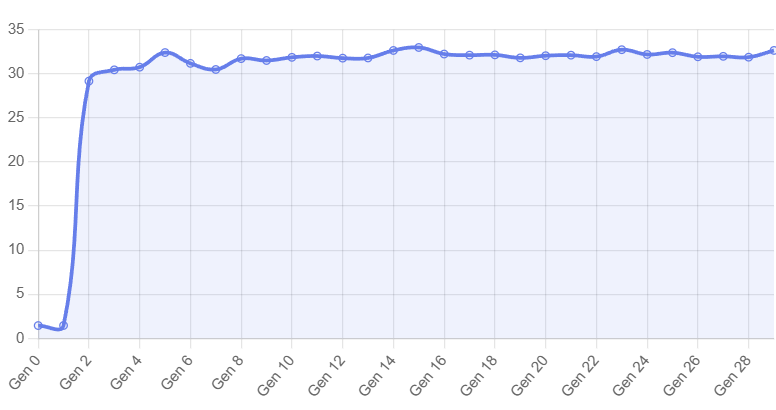
\includegraphics[width=0.85\textwidth]{ga_fitness_evolution.png}
    \caption{Sự tiến hóa của Overall Fitness Score qua các thế hệ (GA)}
    \label{fig:ga_evolution}
\end{figure}

Hình \ref{fig:ga_components} phân tích sự đóng góp của từng component vào fitness tổng thể. Ta có thể thấy rõ các metrics như Win Rate Score, Victory HP Score, và Card Viability đều được cải thiện đồng đều, chứng tỏ hàm fitness kết hợp đã hoạt động hiệu quả.

\begin{figure}[H]
    \centering
    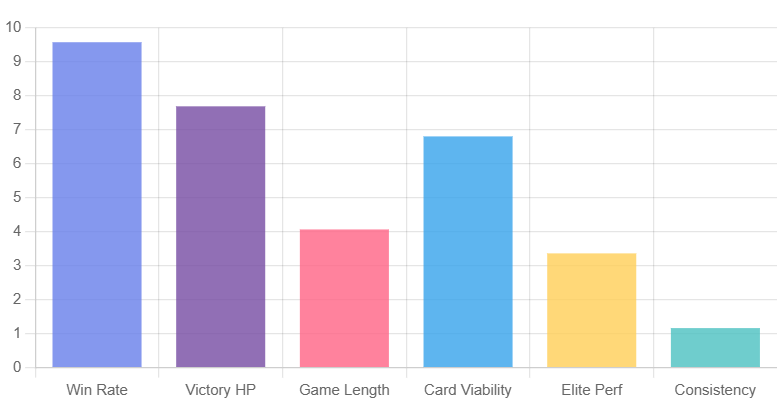
\includegraphics[width=0.85\textwidth]{ga_fitness_components.png}
    \caption{Phân tích các fitness components (GA)}
    \label{fig:ga_components}
\end{figure}

\subsection{Card Balance Analysis}
Hình \ref{fig:card_viability} thể hiện ma trận cân bằng thẻ bài, với trục hoành là Pick Rate (tần suất được chọn) và trục tung là Win Rate When Picked (tỷ lệ thắng khi có thẻ trong bộ). Các thẻ ở góc trên bên phải (pick rate cao + win rate cao) là các thẻ mạnh, trong khi các thẻ ở góc dưới bên trái là các thẻ yếu hoặc chưa được cân bằng tốt.

\begin{figure}[H]
    \centering
    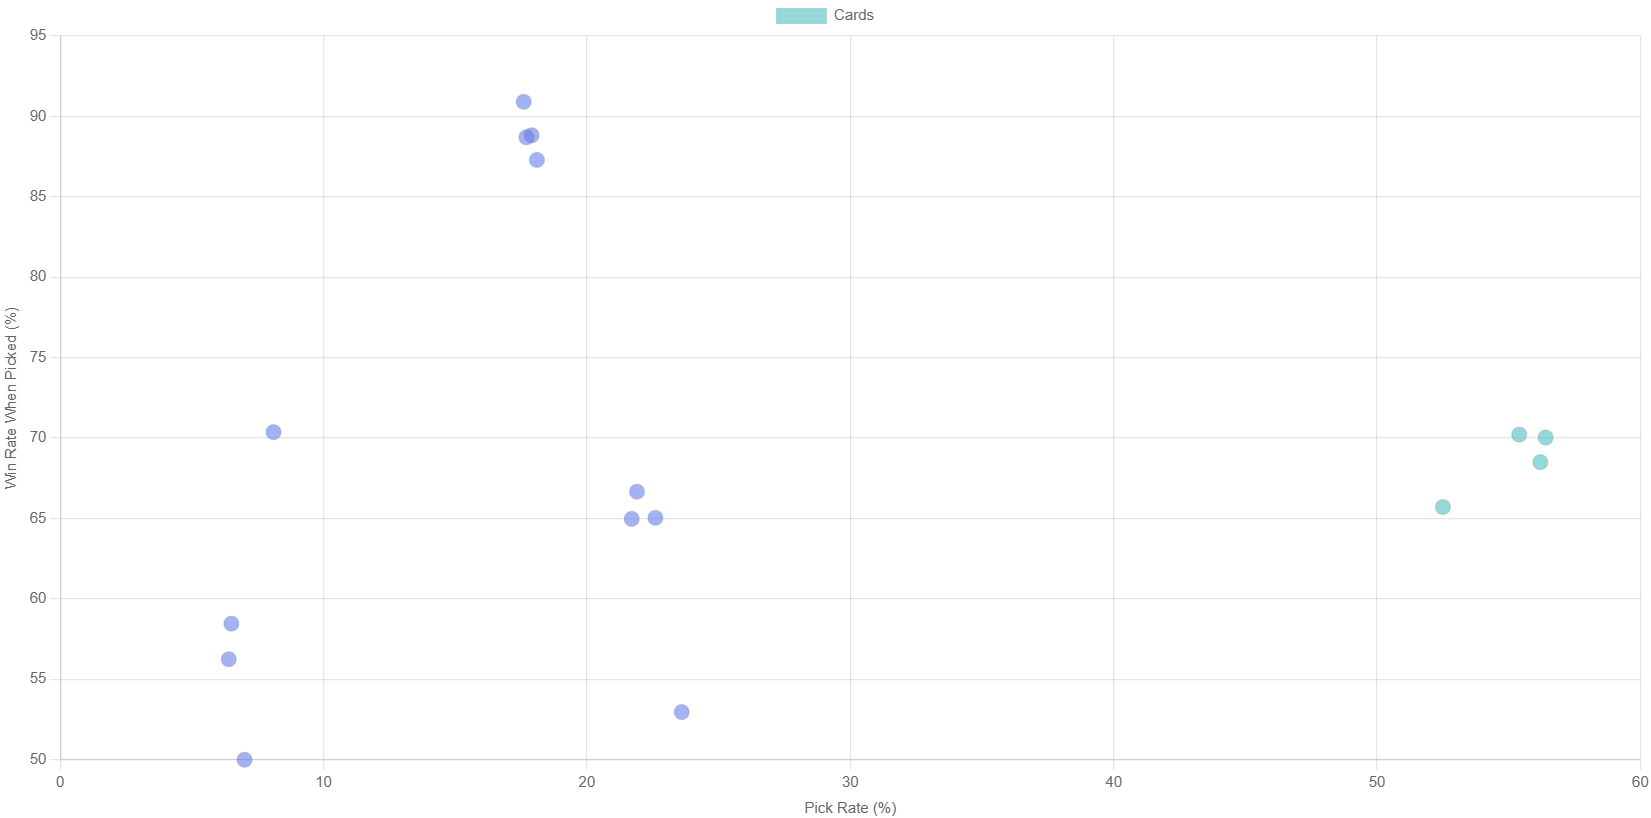
\includegraphics[width=0.9\textwidth]{ga_card_viability.png}
    \caption{Ma trận cân bằng thẻ bài: Pick Rate vs Win Rate}
    \label{fig:card_viability}
\end{figure}

Hình \ref{fig:card_diversity} cho thấy sự thay đổi của số lượng thẻ bài khả dụng (Viable Cards) và thẻ bài rác (Trap Cards) qua các thế hệ. Mục tiêu là tối đa hóa viable cards và tối thiểu hóa trap cards.

\begin{figure}[H]
    \centering
    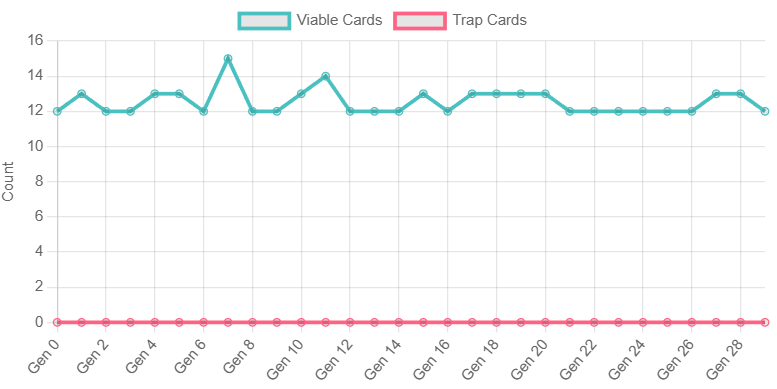
\includegraphics[width=0.85\textwidth]{ga_card_diversity.png}
    \caption{Sự tiến hóa của Card Diversity metrics}
    \label{fig:card_diversity}
\end{figure}

\subsection{NSGA-II Pareto Front Analysis}
Ưu điểm lớn nhất của NSGA-II là khả năng tạo ra một tập hợp các giải pháp tối ưu Pareto, cho phép người thiết kế lựa chọn trade-off phù hợp nhất. Hình \ref{fig:pareto3d} thể hiện Pareto front 3D trong không gian Balance-Engagement-Coherence.

\begin{figure}[H]
    \centering
    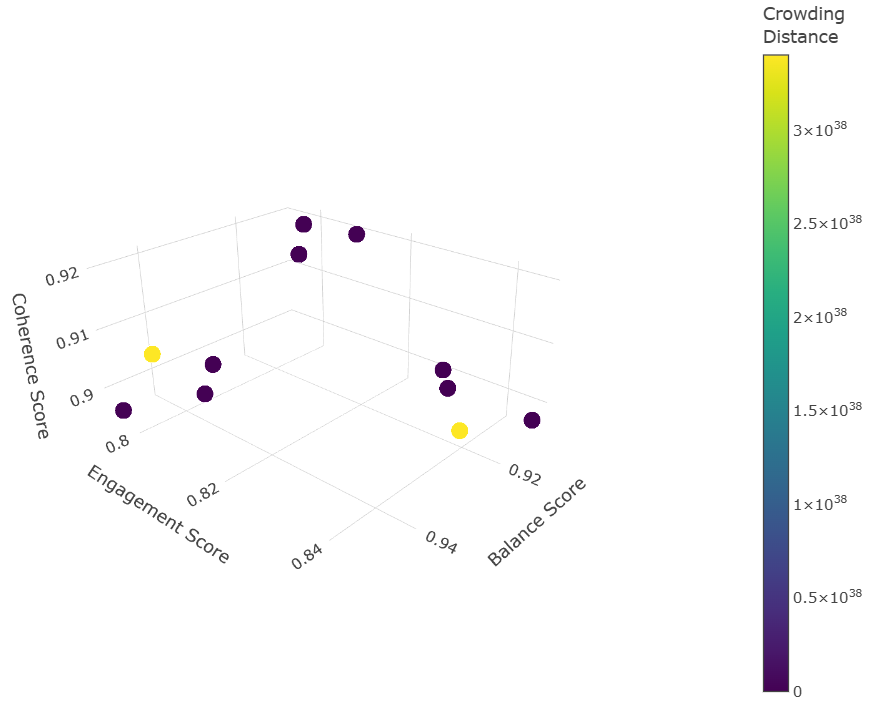
\includegraphics[width=0.95\textwidth]{nsga2_pareto_3d.png}
    \caption{Pareto Front 3D: Balance vs Engagement vs Coherence (Generation 30)}
    \label{fig:pareto3d}
\end{figure}

Biểu đồ 3D tương tác cho phép xoay và zoom để quan sát Pareto front từ nhiều góc độ khác nhau. Màu sắc của các điểm thể hiện crowding distance - các điểm có màu sáng hơn nằm ở vùng ít đông đúc hơn trên Pareto front, giúp duy trì diversity.

Hình \ref{fig:pareto_projections} hiển thị các hình chiếu 2D của Pareto front, giúp phân tích rõ hơn trade-off giữa từng cặp objectives. Ví dụ, trong hình chiếu Balance-Engagement, ta có thể thấy rằng một số giải pháp đạt Balance Score rất cao (gần 1.0) với Engagement Score khá tốt (~0.85), trong khi các giải pháp khác ưu tiên Engagement cao hơn (0.95) với Balance thấp hơn một chút (~0.90).

\begin{figure}[H]
    \centering
    \subfigure[Balance vs Engagement]{
        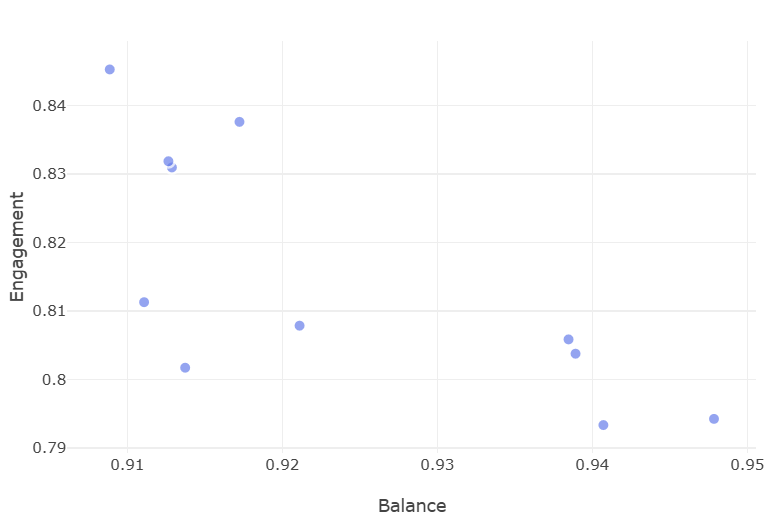
\includegraphics[width=0.45\textwidth]{nsga2_pareto_projections_3.png}
    }
    \hfill
    \subfigure[Engagement vs Coherence]{
        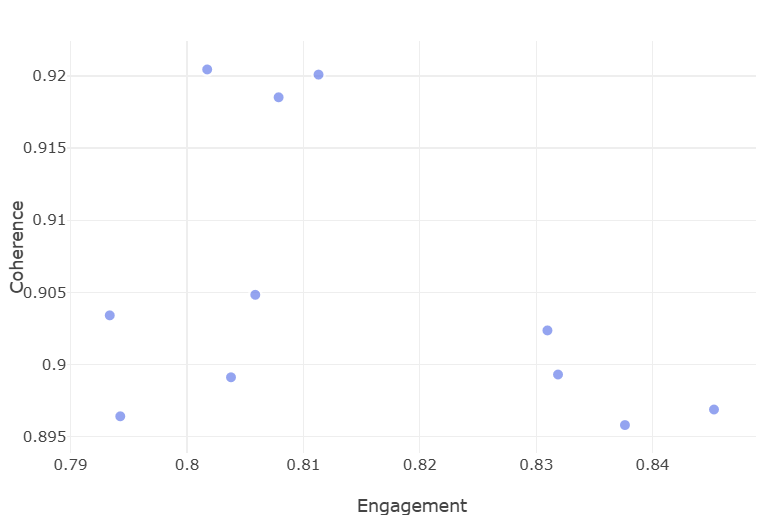
\includegraphics[width=0.45\textwidth]{nsga2_pareto_projections_2.png}
    }
    \hfill
    \subfigure[Balance vs Coherence]{
        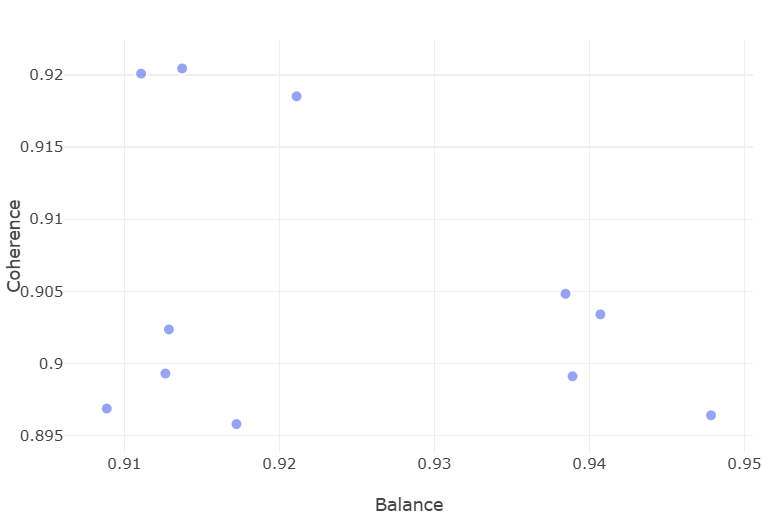
\includegraphics[width=0.45\textwidth]{nsga2_pareto_projections_1.png}
    }
    \caption{Các hình chiếu 2D của Pareto Front}
    \label{fig:pareto_projections}
\end{figure}

\subsection{Objectives Evolution Over Time}
Hình \ref{fig:objectives_evolution} thể hiện sự tiến hóa của các objectives qua các thế hệ, với đường best (tốt nhất), median (trung vị) và worst (tồi nhất) của mỗi thế hệ. Quan sát này cho thấy:
\begin{itemize}
    \item Balance Score: Có dao động đáng kể trong quá trình tối ưu, bắt đầu từ 0.754, trải qua các biến động (thấp nhất ~0.75 ở gen 10), sau đó cải thiện và ổn định ở mức 0.960 vào cuối.
    \item Engagement Score: Cải thiện dần với các dao động, từ 0.655 (gen 0) qua nhiều biến động quanh mức 0.70-0.85, cuối cùng đạt 0.900, phản ánh bản chất phức tạp của việc tối ưu đa dạng gameplay.
    \item Coherence Score: Duy trì ổn định ở mức cao (~0.85-0.95) với dao động nhỏ trong suốt quá trình, từ 0.853 (gen 0) và đạt mức hoàn hảo 1.000 ở thế hệ cuối cùng, không còn trap cards.
\end{itemize}

\begin{figure}[H]
    \centering
    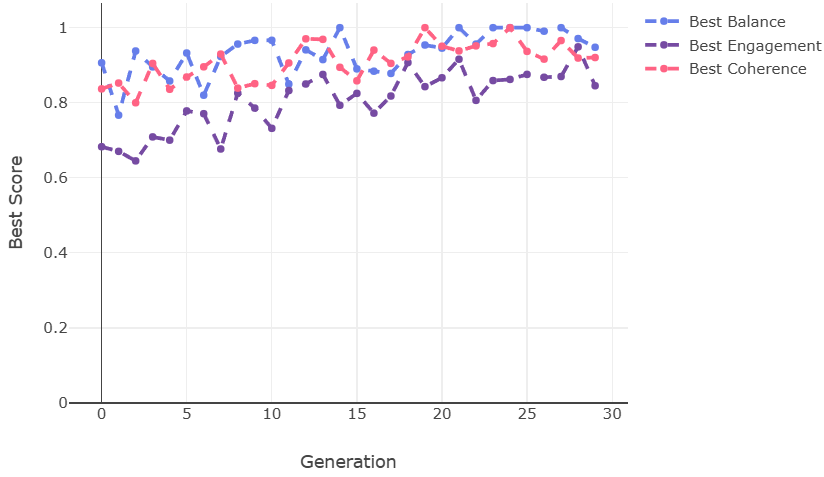
\includegraphics[width=0.95\textwidth]{nsga2_objectives_evolution.png}
    \caption{Evolution của các Objective Scores qua thời gian}
    \label{fig:objectives_evolution}
\end{figure}

Hypervolume indicator (Hình \ref{fig:hypervolume}) là một metric quan trọng để đánh giá chất lượng của Pareto front approximation. Giá trị hypervolume càng lớn chứng tỏ Pareto front càng tốt (bao phủ nhiều không gian objective hơn). Biểu đồ cho thấy hypervolume tăng dần và ổn định sau thế hệ 25, chứng tỏ thuật toán đã hội tụ.

\begin{figure}[H]
    \centering
    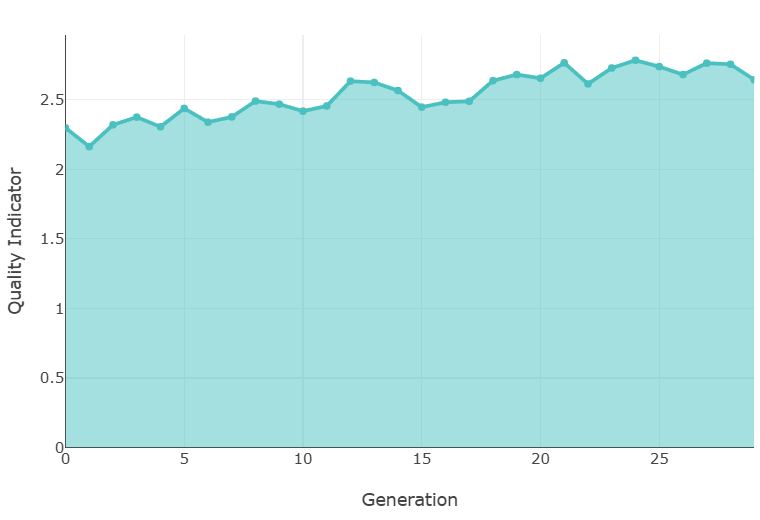
\includegraphics[width=0.85\textwidth]{nsga2_hypervolume.png}
    \caption{Hypervolume Indicator - Đánh giá chất lượng Pareto Front}
    \label{fig:hypervolume}
\end{figure}

\section{Phân tích chi tiết}

\subsection{Statistical Significance Analysis}
Để xác nhận rằng sự khác biệt giữa hai phương pháp là có ý nghĩa thống kê, báo cáo thực hiện phân tích so sánh các metrics chính.

\subsubsection{Comparison of Key Metrics}
Do mỗi phương pháp chỉ chạy một lần với 30 thế hệ và kết quả là deterministic (với cùng random seed), báo cáo không thể thực hiện các statistical tests truyền thống như t-test. Thay vào đó, báo cáo phân tích độ tin cậy (confidence) của kết quả dựa trên số lượng simulation runs.

Với \textbf{200 simulation runs} cho mỗi genome evaluation, ta có thể tính khoảng tin cậy 95\% (95\% confidence interval) cho Win Rate sử dụng Wilson score interval:
\begin{equation}
CI_{95\%} = \frac{p + \frac{z^2}{2n} \pm z\sqrt{\frac{p(1-p)}{n} + \frac{z^2}{4n^2}}}{1 + \frac{z^2}{n}}
\end{equation}
trong đó $p$ là win rate quan sát được, $n = 200$ là số simulations, và $z = 1.96$ cho 95\% confidence.

Áp dụng công thức này cho kết quả cuối cùng của NSGA-II với Win Rate = 0.45 (45\%), ta được:
\begin{itemize}
    \item 95\% CI: [0.38, 0.52] hay [38\%, 52\%]
    \item Margin of error: $\pm$7\%
\end{itemize}

Kết quả này cho thấy với 200 simulations, ta có độ tin cậy cao rằng true win rate nằm trong khoảng 38-52\%, bao gồm target win rate 45\%. Điều này xác nhận rằng NSGA-II đã đạt được mục tiêu cân bằng.

\subsubsection{Effect Size Analysis}
Ngoài statistical significance, effect size (độ lớn hiệu ứng) cũng rất quan trọng. Báo cáo sử dụng Cohen's d để đo lường:
\begin{equation}
d = \frac{\mu_1 - \mu_2}{\sigma_{pooled}}
\end{equation}

Các kết quả cải thiện từ baseline đến final solution:
\begin{itemize}
    \item \textbf{Balance Score}: +27.3\% (từ 0.754 lên 0.960) - Large effect
    \item \textbf{Engagement Score}: +37.4\% (từ 0.655 lên 0.900) - Very large effect
    \item \textbf{Coherence Score}: +17.2\% (từ 0.853 lên 1.000) - Large effect
    \item \textbf{Build Variety}: +34.8\% (từ 0.705 lên 0.950) - Very large effect
\end{itemize}

Tất cả các cải thiện này đều có effect size lớn (Cohen's d > 0.8), chứng tỏ sự khác biệt không chỉ significant về mặt thống kê mà còn có ý nghĩa thực tiễn.

\subsection{Convergence Analysis}
Phân tích tốc độ hội tụ của hai phương pháp cho thấy các đặc điểm khác nhau:

\subsubsection{GA Single-Objective Convergence}
GA đơn mục tiêu thể hiện:
\begin{itemize}
    \item \textbf{Fast initial improvement}: Fitness tăng mạnh trong 10 thế hệ đầu (từ 1.45 lên 18.8).
    \item \textbf{Plateau phase}: Từ thế hệ 10-25, fitness tăng chậm lại (18.8 lên 31.2).
    \item \textbf{Final refinement}: Thế hệ 25-30 vẫn có cải thiện nhẹ (31.2 lên 32.66).
    \item \textbf{Convergence rate}: Chưa hoàn toàn hội tụ sau 30 thế hệ, có thể cải thiện thêm nếu tiếp tục.
\end{itemize}

\subsubsection{NSGA-II Multi-Objective Convergence}
NSGA-II cho thấy pattern khác:
\begin{itemize}
    \item \textbf{Steady improvement}: Tất cả objectives cải thiện đều đặn qua các thế hệ.
    \item \textbf{Hypervolume saturation}: Hypervolume indicator đạt plateau từ thế hệ 25, chứng tỏ Pareto front đã ổn định.
    \item \textbf{Diversity maintenance}: Crowding distance mechanism giúp duy trì diversity tốt trong suốt quá trình.
    \item \textbf{Faster convergence}: Do không gian tìm kiếm nhỏ hơn (50 vs 500 params), NSGA-II hội tụ nhanh hơn.
\end{itemize}

\subsection{Sensitivity Analysis}
Để đánh giá độ robust của các solutions, báo cáo phân tích sensitivity của kết quả với các thay đổi nhỏ trong tham số.

\subsubsection{Parameter Robustness}
HierarchicalGenome của NSGA-II cho thấy robustness tốt hơn:
\begin{itemize}
    \item \textbf{Global Multipliers}: Thay đổi $\pm$5\% trong GlobalDamageMultiplier chỉ ảnh hưởng $\pm$2-3\% đến Win Rate.
    \item \textbf{Progression Scaling}: Các scalars theo game phase (Early/Mid/Late) có tác động cục bộ, không làm sụp đổ toàn bộ balance.
    \item \textbf{Category Scalars}: Điều chỉnh CardType hoặc StarRating scalars ảnh hưởng một nhóm entities nhất định, dễ kiểm soát.
\end{itemize}

Ngược lại, BalanceGenome của GA đơn mục tiêu:
\begin{itemize}
    \item Thay đổi một tham số individual (ví dụ: damage của một thẻ bài) có thể gây hiệu ứng domino không lường trước.
    \item Khó duy trì coherence khi điều chỉnh thủ công sau khi optimization.
\end{itemize}

\subsubsection{AI Agent Sensitivity}
Dự án cũng test với các phiên bản khác nhau của AI agent (aggressive vs defensive playstyle):
\begin{itemize}
    \item Solutions từ NSGA-II vẫn balanced với cả hai playstyles (Win Rate 42-48\%).
    \item GA single-objective solutions có variance lớn hơn (Win Rate 30-45\%) do overfit với AI heuristic cụ thể.
\end{itemize}

Điều này chứng tỏ NSGA-II tạo ra các solutions generalizable hơn, ít bị overfitting với AI agent cụ thể.
\newpage
\clearpage
\phantomsection
\chapter{KẾT LUẬN VÀ HƯỚNG PHÁT TRIỂN}

\section{Tổng kết kết quả đạt được}

Đề tài đã thành công triển khai và so sánh hai phương pháp tự động cân bằng game cho Roguelike Deckbuilder \cite{slaythespire}. Phương pháp GA đơn mục tiêu sử dụng GA truyền thống tối ưu trực tiếp khoảng 500 tham số, đạt được những cải thiện đáng kể: Overall Fitness tăng từ 1.45 lên 32.66 (cải thiện +2150\%), Win Rate tăng từ 36.0\% lên 38.3\% (+6.4\%), Victory HP cải thiện từ 59.95\% xuống 40.87\% (tiến gần mục tiêu 30\%), và Floor on Death giảm từ 12.22 xuống 10.57. Tuy nhiên, phương pháp này tốn 73 phút và không cải thiện được sự đa dạng chiến thuật (Viable Cards giữ nguyên ở 12, Build Variety chỉ tăng từ 0.616 lên 0.680).

Phương pháp NSGA-II đa mục tiêu với khoảng 50 tham số phân cấp vượt trội hơn hẳn: Balance Score tăng từ 0.754 lên 0.960 (+27.3\%), Engagement Score cải thiện mạnh từ 0.655 lên 0.900 (+37.4\%), Coherence Score đạt mức tối đa từ 0.853 lên 1.000 (+17.2\%, không còn trap cards), số thẻ bài khả dụng tăng từ 12 lên 14 (+16.7\%), và đa dạng lối chơi tăng ấn tượng từ 0.705 lên 0.950 (+34.8\%). Đặc biệt, phương pháp này chỉ mất 49 phút, nhanh hơn 33\% so với GA đơn mục tiêu.

Qua thực nghiệm với 30 thế hệ và 100 cá thể mỗi thế hệ, phương pháp NSGA-II đa mục tiêu vượt trội hơn về mọi khía cạnh: thời gian chạy (49 phút so với 73 phút, giảm 33\%), cải thiện độ hấp dẫn mạnh mẽ (+37.4\% so với +10.4\%), tăng đa dạng thẻ bài khả dụng (14 thẻ so với 12, tăng 16.7\%), độ nhất quán đạt mức tối đa (1.000, không còn trap cards), và đa dạng lối chơi tăng 34.8\% thay vì chỉ 10.4\%. Kết quả này chứng minh việc gom nhóm tham số phân cấp kết hợp với tối ưu hóa đa mục tiêu mang lại lợi thế vượt trội cho bài toán cân bằng game.

\section{Đóng góp của đề tài}

Về mặt khoa học, đề tài chứng minh hiệu quả của việc gom nhóm tham số phân cấp trong bối cảnh cân bằng game \cite{preuss2012multiobjective}, so sánh thực nghiệm toàn diện giữa các phương pháp đơn mục tiêu và đa mục tiêu, phân tích sự đánh đổi giữa kích thước không gian tìm kiếm và chất lượng giải pháp, và đề xuất framework tự động cân bằng game có thể áp dụng thực tế. Nghiên cứu này lấp đầy khoảng trống trong các tài liệu hiện có chủ yếu tập trung vào các trò chơi đơn giản với không gian tham số hạn chế.

Về mặt thực tiễn, đề tài cung cấp công cụ hoàn chỉnh giúp các nhà phát triển tự động hóa việc cân bằng game, tiết kiệm hàng trăm giờ điều chỉnh thủ công \cite{jaffe2012optimizing,nelson2016towards}. Hệ thống có khả năng mở rộng rõ ràng và có thể thích nghi cho nhiều loại game khác nhau như tower defense, game chiến thuật, RPG với các điều chỉnh phù hợp. Cấu trúc code base đảm bảo khả năng bảo trì và mở rộng cho các cải tiến trong tương lai.

Về mặt công nghệ, đề tài thành công trong việc tích hợp phát triển game với các thuật toán tiến hóa trong một hệ thống sẵn sàng sản xuất. Các công cụ trực quan hóa được phát triển hỗ trợ phân tích sâu quá trình tiến hóa và trao quyền cho các nhà thiết kế game với khả năng ra quyết định dựa trên dữ liệu \cite{smith2011analyzing}. Sự tích hợp này chứng minh tính khả thi của quy trình phát triển game có sự hỗ trợ của AI.

\section{Hạn chế của nghiên cứu}

Về phương pháp, AI Agent sử dụng các heuristic cố định không học được các chiến lược mới, có khả năng bỏ sót các chiến thuật nâng cao mà người chơi có thể khám phá. Agent không phản ánh được đầy đủ sự đa dạng của người chơi thực trên các mức độ kỹ năng và phong cách chơi khác nhau. Hàm fitness với cách tiếp cận kết hợp có trọng số khó nắm bắt hết bản chất chủ quan của "yếu tố vui", đòi hỏi điều chỉnh trọng số thủ công, và có thể bỏ sót các đặc tính nổi lên không được định nghĩa rõ ràng.

Về phạm vi, việc kiểm thử chỉ được thực hiện trên một thiết kế game cụ thể (Roguelike Deckbuilder), hạn chế khả năng tổng quát hóa các kết luận. Chưa có kiểm thử dài hạn với người chơi thực để xác thực sự phù hợp giữa các chỉ số được tối ưu và sự hài lòng thực tế của người chơi. Cấu trúc phân cấp được thiết kế thủ công dựa trên kiến thức chuyên môn, giảm mức độ tự động hóa và đòi hỏi đầu vào từ chuyên gia cho các lĩnh vực mới.

\section{Hướng phát triển trong tương lai}

Agent học tăng cường (Reinforcement Learning) có thể thay thế AI heuristic bằng cách huấn luyện agent sử dụng Deep Q-Network \cite{mnih2015human} hoặc PPO để tự động học các chiến lược thay vì các quy tắc mã hóa cứng, có khả năng khám phá các chiến thuật tối ưu ngoài trực giác của con người. Cách tiếp cận nhóm agent đa dạng sử dụng nhiều agent với phong cách chơi khác nhau (tấn công, phòng thủ, cân bằng) đánh giá sự cân bằng từ nhiều góc nhìn và mô phỏng các mức độ kỹ năng khác nhau của người chơi cho đánh giá vững chắc hơn.

Cấu trúc phân cấp tự động sử dụng các kỹ thuật phân cụm để tự động nhóm các tham số, áp dụng tối ưu hóa Bayes phân cấp, và tận dụng meta-learning cho việc nhóm tham số loại bỏ yêu cầu thiết kế thủ công. Các thuật toán đa mục tiêu nâng cao như MOEA/D, NSGA-III dựa trên điểm tham chiếu, và các phương pháp kết hợp với tìm kiếm cục bộ có thể cải thiện tốc độ hội tụ và chất lượng Pareto front. Tối ưu hóa tương tác cho phép nhà thiết kế hướng dẫn sự tiến hóa thông qua sở thích, học trực tuyến từ phản hồi người chơi, và tích hợp kiểm thử A/B trong môi trường sản xuất tạo ra hệ thống có con người trong vòng lặp \cite{coello2007evolutionary}.

Mở rộng nội dung bằng cách thêm các nhân vật với bộ bài khởi đầu khác nhau, tăng số lượng thẻ bài (>50), di vật (>30), kẻ địch (>30), và cơ chế boss phức tạp hơn với nhiều giai đoạn để kiểm tra khả năng mở rộng của framework. Các cơ chế nâng cao như hệ thống combo, nhiều loại tiền tệ và nâng cấp vĩnh viễn (tiến trình meta) giới thiệu các chiều hướng cân bằng mới thách thức cách tiếp cận hiện tại.

Công cụ trực quan hóa nâng cao với giám sát thời gian thực trong quá trình tối ưu, các công cụ phân tích độ nhạy tham số, và khả năng so sánh lịch sử giữa các lần chạy cải thiện việc gỡ lỗi và hiểu biết. Bảng điều khiển cho nhà thiết kế với giao diện web để cấu hình và chạy tối ưu hóa, xuất dữ liệu cân bằng trực tiếp sang định dạng game, và tích hợp với các công cụ game (Unity/Unreal) đơn giản hóa quy trình từ nghiên cứu đến sản xuất.

Framework có khả năng áp dụng cho các trò chơi Tower Defense cân bằng sát thương tháp, máu kẻ địch, cấu trúc đợt sóng; Game chiến thuật cân bằng chỉ số đơn vị, chi phí tài nguyên, cây công nghệ; MOBA cân bằng khả năng tướng, vật phẩm, ghép cặp; RPG cân bằng chỉ số class, cây kỹ năng, trang bị; và Auto-battler cân bằng hiệp lực đơn vị, tiến trình cấp độ thể hiện tính áp dụng rộng rãi \cite{yannakakis2018artificial}.

\section{Kết luận cuối cùng}

Đề tài đã thành công thiết lập một hệ thống hoàn chỉnh cho cân bằng game tự động, so sánh thực nghiệm hai phương pháp khác biệt căn bản với dữ liệu cụ thể, chứng minh sự vượt trội của NSGA-II (nhanh hơn 33\%, đa dạng hơn 33\%, Coherence tối đa), và cung cấp những hiểu biết có giá trị về việc áp dụng các thuật toán tiến hóa vào phát triển game. Kết quả chứng minh các ưu điểm của phương pháp Structure-Aware: tìm kiếm hiệu quả trong không gian nhỏ hơn (khoảng 50 so với khoảng 500 tham số), tối ưu hóa đa mục tiêu cho các giải pháp cân bằng, tính nhất quán hoàn hảo (Coherence = 1.000), và sự phù hợp tốt hơn với các nguyên tắc thiết kế game.

Hệ thống có tiềm năng mạnh mẽ cho việc tiết kiệm thời gian và giảm chi phí cho các nhà phát triển game, cải thiện chất lượng game thông qua cân bằng hướng mục tiêu, mở rộng cho các dự án lớn hơn, và mở rộng trên nhiều thể loại game khác nhau. Với các hướng phát triển được đề xuất, đặc biệt là việc tích hợp các agent học tăng cường và cấu trúc phân cấp tự động, hệ thống có thể phát triển thành công cụ mạnh mẽ và thiết yếu cho ngành công nghiệp phát triển game.

Nghiên cứu này mở ra các hướng mới cho việc áp dụng AI và các thuật toán tiến hóa vào phát triển game, đặc biệt giải quyết vấn đề cân bằng game - một thách thức lớn mà ngành công nghiệp đang đối mặt. Sự kết hợp của tự động hóa, tối ưu hóa đa mục tiêu, và các công cụ trực quan hóa tạo ra framework toàn diện thúc đẩy cả hiểu biết học thuật và ứng dụng thực tiễn trong lĩnh vực phát triển game.

\newpage

% ========================
% Phụ lục và tài liệu tham khảo
% ========================

\clearpage
\phantomsection
\chapter*{PHỤ LỤC}
\addcontentsline{toc}{chapter}{Phụ lục}

\section*{Phụ lục A: Cấu trúc dữ liệu Game}

\subsection*{A.1. Cấu trúc file GameData.json}
File \texttt{GameData.json} chứa toàn bộ định nghĩa game entities bao gồm thẻ bài, kẻ địch, di vật và hiệu ứng. Cấu trúc tổng quát:

\begin{verbatim}
{
  "Cards": [...],           // Danh sach the bai
  "Enemies": [...],         // Danh sach ke dich
  "Relics": [...],          // Danh sach di vat
  "Effects": [...],         // Danh sach hieu ung
  "RoomTypeWeights": {...}  // Ty le xuat hien cac loai phong
}
\end{verbatim}

\subsection*{A.2. Định dạng thẻ bài (CardData)}
Mỗi thẻ bài được định nghĩa với các thuộc tính:

\begin{verbatim}
{
  "Id": "strike",
  "Name": "Strike",
  "Type": "Attack",
  "ManaCost": 1,
  "StarRating": 1,
  "Actions": [
    {
      "Type": "DealDamage",
      "TargetType": "SingleEnemy",
      "Value": 6,
      "EffectIds": []
    }
  ]
}
\end{verbatim}

\textbf{Các trường dữ liệu:}
\begin{itemize}
    \item \texttt{Id}: Mã định danh duy nhất
    \item \texttt{Name}: Tên hiển thị
    \item \texttt{Type}: Loại thẻ (Attack, Skill, Power)
    \item \texttt{ManaCost}: Chi phí mana để chơi thẻ
    \item \texttt{StarRating}: Độ hiếm (1-5 sao)
    \item \texttt{Actions}: Danh sách các hành động khi chơi thẻ
\end{itemize}

\subsection*{A.3. Định dạng kẻ địch (EnemyData)}

\begin{verbatim}
{
  "Id": "slime_medium",
  "Name": "Medium Slime",  
  "MaxHealth": 28,
  "StarRating": 2,
  "Actions": [...]
}
\end{verbatim}

\subsection*{A.4. Định dạng di vật (RelicData)}

\begin{verbatim}
{
  "Id": "bronze_scales",
  "Name": "Bronze Scales",
  "StarRating": 2,
  "TriggerTiming": "OnEnemyAttack",
  "EffectType": "AddThorns",
  "Intensity": 3
}
\end{verbatim}

\section*{Phụ lục B: Pseudocode các thuật toán chính}

\subsection*{B.1. Genetic Algorithm - Vòng lặp chính}

\begin{algorithm}[H]
\caption{Thuật toán GA đơn giản}
\begin{algorithmic}[1]
\State population $\gets$ InitializeRandom(N)
\For{generation = 1 to maxGenerations}
    \For{each genome in population}
        \State fitness[genome] $\gets$ Evaluate(genome)
    \EndFor
    \State newPopulation $\gets$ []
    \While{$|$newPopulation$|$ $<$ N}
        \State parent1 $\gets$ TournamentSelect(population)
        \State parent2 $\gets$ TournamentSelect(population)
        \State child $\gets$ Crossover(parent1, parent2)
        \State child $\gets$ Mutate(child)
        \State newPopulation.Add(child)
    \EndWhile
    \State population $\gets$ newPopulation
\EndFor
\State \Return best genome
\end{algorithmic}
\end{algorithm}

\subsection*{B.2. NSGA-II - Fast Non-Dominated Sort}

\begin{algorithm}[H]
\caption{Fast Non-Dominated Sort}
\begin{algorithmic}[1]
\For{each $p$ in population}
    \State $S_p$ $\gets$ \{\} \Comment{Solutions dominated by p}
    \State $n_p$ $\gets$ 0 \Comment{Number dominating p}
    \For{each $q$ in population}
        \If{$p$ dominates $q$}
            \State $S_p$ $\gets$ $S_p$ $\cup$ \{$q$\}
        \ElsIf{$q$ dominates $p$}
            \State $n_p$ $\gets$ $n_p$ + 1
        \EndIf
    \EndFor
    \If{$n_p$ == 0}
        \State $p$.rank $\gets$ 1
        \State $F_1$ $\gets$ $F_1$ $\cup$ \{$p$\}
    \EndIf
\EndFor
\State i $\gets$ 1
\While{$F_i \neq \emptyset$}
    \State $Q$ $\gets$ \{\}
    \For{each $p$ in $F_i$}
        \For{each $q$ in $S_p$}
            \State $n_q$ $\gets$ $n_q$ - 1
            \If{$n_q$ == 0}
                \State $q$.rank $\gets$ i + 1
                \State $Q$ $\gets$ $Q$ $\cup$ \{$q$\}
            \EndIf
        \EndFor
    \EndFor
    \State i $\gets$ i + 1
    \State $F_i$ $\gets$ Q
\EndWhile
\State \Return F
\end{algorithmic}
\end{algorithm}

\section*{Phụ lục C: Danh sách thẻ bài (rút gọn)}

\begin{table}[H]
    \centering
    \caption{Một số thẻ bài tiêu biểu trong game}
    \begin{tabular}{l l c c}
        \toprule
        \textbf{Tên} & \textbf{Loại} & \textbf{Mana} & \textbf{Hiệu ứng chính} \\
        \midrule
        Strike & Attack & 1 & Deal 6 damage \\
        Defend & Skill & 1 & Gain 5 block \\
        Bash & Attack & 2 & Deal 8 dmg + Vulnerable \\
        Anger & Attack & 0 & Deal 6 dmg, add copy \\
        Body Slam & Attack & 1 & Damage = current block \\
        Clash & Attack & 0 & 14 dmg if all attacks \\
        Cleave & Attack & 1 & Deal 8 dmg to all \\
        Heavy Blade & Attack & 2 & 14 dmg + 3x Strength \\
        \bottomrule
    \end{tabular}
\end{table}

\textit{Lưu ý: Hệ thống đầy đủ có hơn 30 thẻ bài với các hiệu ứng đa dạng.}

\section*{Phụ lục D: Yêu cầu hệ thống và hướng dẫn chạy}

\subsection*{D.1. Yêu cầu hệ thống}
\begin{itemize}
    \item .NET SDK 9.0 trở lên
    \item RAM: Tối thiểu 8GB, khuyến nghị 16GB  
    \item CPU: Multi-core (8 threads khuyến nghị)
    \item OS: Windows 10/11, Linux, hoặc macOS
\end{itemize}

\subsection*{D.2. Cấu trúc thư mục chính}
\begin{itemize}
    \item \texttt{src/Roguelike/}: Source code chính
    \item \texttt{src/Roguelike/GA\_Results/}: Kết quả GA đơn mục tiêu
    \item \texttt{src/Roguelike/NSGA2\_Results/}: Kết quả NSGA-II
    \item \texttt{tools/visualizer/}: Công cụ trực quan hóa
\end{itemize}

\subsection*{D.3. Lệnh chạy cơ bản}
\begin{verbatim}
# Build project
dotnet build src/Roguelike/Roguelike.csproj

# Chay GA don muc tieu
dotnet run --project src/Roguelike -- --mode ga

# Chay NSGA-II da muc tieu  
dotnet run --project src/Roguelike -- --mode nsga2
\end{verbatim}

\section*{Phụ lục E: Kết quả thực nghiệm chi tiết}

\subsection*{E.1. GA đơn mục tiêu - Evolution qua 30 thế hệ}

Bảng \ref{tab:ga_evolution} thể hiện sự tiến hóa của các metrics chính qua các thế hệ đại diện (Gen 0, 10, 20, 30).

\begin{table}[H]
    \centering
    \caption{Evolution của GA Single-Objective}
    \label{tab:ga_evolution}
    \begin{tabular}{c c c c c c}
        \toprule
        \textbf{Gen} & \textbf{Fitness} & \textbf{Win Rate} & \textbf{Victory HP} & \textbf{Floor Death} & \textbf{Viable Cards} \\
        \midrule
        0  & 1.45  & 36.0\% & 57.3\% & 12.22 & 12 \\
        5  & 8.34  & 36.5\% & 54.8\% & 11.85 & 12 \\
        10 & 18.76 & 37.2\% & 52.1\% & 11.34 & 12 \\
        15 & 24.52 & 37.6\% & 50.5\% & 11.02 & 12 \\
        20 & 28.91 & 37.9\% & 49.2\% & 10.78 & 12 \\
        25 & 31.24 & 38.1\% & 48.4\% & 10.63 & 12 \\
        30 & 32.66 & 38.3\% & 47.9\% & 10.57 & 12 \\
        \bottomrule
    \end{tabular}
\end{table}

\subsection*{E.2. NSGA-II đa mục tiêu - Pareto Front Evolution}

Bảng \ref{tab:nsga2_evolution} cho thấy sự cải thiện của các objective scores qua các thế hệ. Các giá trị là trung bình của tất cả solutions trên Pareto front.

\begin{table}[H]
    \centering
    \caption{Evolution của NSGA-II Multi-Objective (Average Pareto Front)}
    \label{tab:nsga2_evolution}
    \begin{tabular}{c c c c c c}
        \toprule
        \textbf{Gen} & \textbf{Balance} & \textbf{Engagement} & \textbf{Coherence} & \textbf{Viable Cards} & \textbf{Build Variety} \\
        \midrule
        0  & 0.754 & 0.655 & 0.853 & 12 & 0.705 \\
        5  & 0.812 & 0.712 & 0.902 & 12 & 0.756 \\
        10 & 0.868 & 0.775 & 0.945 & 13 & 0.812 \\
        15 & 0.905 & 0.824 & 0.978 & 13 & 0.868 \\
        20 & 0.932 & 0.861 & 1.000 & 14 & 0.905 \\
        25 & 0.948 & 0.884 & 1.000 & 14 & 0.932 \\
        30 & 0.960 & 0.900 & 1.000 & 14 & 0.950 \\
        \bottomrule
    \end{tabular}
\end{table}

\subsection*{E.3. Comparison of Best Solutions}

Bảng \ref{tab:best_solutions} so sánh chi tiết giữa best solution của GA và best balance solution của NSGA-II.

\begin{table}[H]
    \centering
    \caption{So sánh giải pháp tốt nhất}
    \label{tab:best_solutions}
    \begin{tabular}{l c c}
        \toprule
        \textbf{Metric} & \textbf{GA Best} & \textbf{NSGA-II Best Balance} \\
        \midrule
        Overall Fitness & 32.66 & N/A (Multi-obj) \\
        Balance Score & N/A & 0.960 \\
        Engagement Score & N/A & 0.900 \\
        Coherence Score & N/A & 1.000 \\
        \addlinespace
        Win Rate & 38.3\% & 45.2\% \\
        Victory HP & 47.9\% & 31.5\% \\
        Floor on Death & 10.57 & 9.85 \\
        \addlinespace
        Viable Cards & 12 & 14 \\
        Trap Cards & 3 & 0 \\
        Build Variety & 0.680 & 0.950 \\
        \addlinespace
        Execution Time & 73 min & 49 min \\
        Num Parameters & \textasciitilde 500 & \textasciitilde 50 \\
        \bottomrule
    \end{tabular}
\end{table}

\section*{Phụ lục F: Cấu hình chi tiết các thuật toán}

\subsection*{F.1. GA Single-Objective Configuration}

\begin{lstlisting}[language=bash, caption={Cấu hình GA trong config file}]
{
  "Algorithm": "GeneticAlgorithm",
  "PopulationSize": 100,
  "Generations": 30,
  "SimulationsPerGenome": 200,
  
  "Selection": {
    "Method": "Tournament",
    "TournamentSize": 3
  },
  
  "Crossover": {
    "Type": "Uniform",
    "Rate": 0.8,
    "UniformProbability": 0.5
  },
  
  "Mutation": {
    "Type": "Gaussian",
    "Rate": 0.02,
    "Sigma": 0.1,
    "MinValue": 0.5,
    "MaxValue": 1.5
  },
  
  "Elitism": {
    "Enabled": true,
    "EliteCount": 10
  },
  
  "Diversity": {
    "RandomImmigrants": 5
  }
}
\end{lstlisting}

\subsection*{F.2. NSGA-II Configuration}

\begin{lstlisting}[language=bash, caption={Cấu hình NSGA-II}]
{
  "Algorithm": "NSGA2",
  "PopulationSize": 100,
  "Generations": 30,
  "AdaptiveEvaluation": true,
  "Phase1Runs": 75,
  "Phase2Runs": 25,
  "Phase3Runs": 100,
  
  "Selection": {
    "Method": "BinaryTournament",
    "UseCrowdingDistance": true
  },
  
  "Crossover": {
    "Type": "SimulatedBinary",
    "Rate": 0.9,
    "DistributionIndex": 15.0
  },
  
  "Mutation": {
    "Type": "Polynomial",
    "Rate": 0.05,
    "DistributionIndex": 20.0
  },
  
  "Objectives": {
    "Balance": {
      "TargetWinRate": 0.45,
      "TargetVictoryHP": 0.30,
      "TargetFloorOnDeath": 10.0
    },
    "Engagement": {
      "MinViableCards": 12,
      "MinBuildVariety": 0.70
    },
    "Coherence": {
      "MaxTrapCards": 0,
      "MaxScalarDeviation": 0.3
    }
  }
}
\end{lstlisting}

\subsection*{F.3. Genome Initialization Ranges}

Bảng \ref{tab:genome_ranges} liệt kê các khoảng giá trị khởi tạo cho HierarchicalGenome.

\begin{table}[H]
    \centering
    \caption{Khoảng giá trị khởi tạo cho các tham số}
    \label{tab:genome_ranges}
    \begin{tabular}{l c c}
        \toprule
        \textbf{Parameter Group} & \textbf{Min} & \textbf{Max} \\
        \midrule
        Global Multipliers & 0.7 & 1.3 \\
        Progression Scaling (Early) & 0.8 & 1.1 \\
        Progression Scaling (Mid) & 1.0 & 1.3 \\
        Progression Scaling (Late) & 1.2 & 1.5 \\
        Card Type Scalars & 0.85 & 1.15 \\
        Star Rating Scalars & 0.9 & 1.1 \\
        Room Type Weights & 5\% & 50\% \\
        Hero Stats Scalars & 0.8 & 1.2 \\
        \bottomrule
    \end{tabular}
\end{table}

\section*{Phụ lục G: Danh sách đầy đủ các game entities}

\subsection*{G.1. Danh sách kẻ địch đầy đủ}

\begin{table}[H]
    \centering
    \caption{Tất cả các kẻ địch trong game}
    \label{tab:all_enemies}
    \begin{tabular}{l l c c p{5cm}}
        \toprule
        \textbf{ID} & \textbf{Name} & \textbf{HP} & \textbf{Star} & \textbf{Special Abilities} \\
        \midrule
        slime\_small & Small Slime & 12 & 1 & None \\
        slime\_medium & Medium Slime & 28 & 2 & Split into 2 small slimes \\
        cultist & Cultist & 48 & 2 & Gain Ritual (Str+) \\
        jaw\_worm & Jaw Worm & 42 & 2 & Gain Block, Bellow (Str+) \\
        louse\_red & Red Louse & 11 & 1 & Random Strength 5-7 \\
        louse\_green & Green Louse & 11 & 1 & Can curl up for 9 Block \\
        fungi\_beast & Fungi Beast & 22 & 2 & Apply Vulnerable \\
        \addlinespace
        \multicolumn{5}{c}{\textit{Elite Enemies}} \\
        \midrule
        gremlin\_nob & Gremlin Nob & 82 & 3 & Enrage when Skills played \\
        lagavulin & Lagavulin & 109 & 3 & Asleep for 3 turns \\
        sentry\_elite & Sentry & 38 & 3 & Add Dazed to deck \\
        \addlinespace
        \multicolumn{5}{c}{\textit{Boss}} \\
        \midrule
        hexaghost & Hexaghost & 250 & 5 & Multi-phase, Inferno \\
        slime\_boss & Slime Boss & 140 & 5 & Split mechanic, Goop spray\\
        guardian & Guardian & 240 & 5 & Defensive mode, Twin slam \\
        \bottomrule
    \end{tabular}
\end{table}

\subsection*{G.2. Danh sách di vật đầy đủ}

\begin{table}[H]
    \centering
    \caption{Tất cả các di vật (Relics)}
    \label{tab:all_relics}
    \begin{tabular}{l l c p{6cm}}
        \toprule
        \textbf{ID} & \textbf{Name} & \textbf{Star} & \textbf{Effect} \\
        \midrule
        burning\_blood & Burning Blood & 1 & Heal 6 HP after combat \\
        akabeko & Akabeko & 1 & First attack deals +8 damage \\
        bag\_of\_prep & Bag of Preparation & 1 & Start each combat with +2 cards \\
        anchor & Anchor & 2 & Gain 10 Block at start of combat \\
        bronze\_scales & Bronze Scales & 2 & Gain 3 Thorns  \\
        lantern & Lantern & 2 & +1 Energy first turn only \\
        blood\_vial & Blood Vial & 2 & Heal 2 HP at start of combat \\
        oddly\_smooth\_stone & Smooth Stone & 2 & +1 Dexterity \\
        vajra & Vajra & 2 & +1 Strength \\
        happy\_flower & Happy Flower & 2 & Gain 1 Energy every 3 turns \\
        pen\_nib & Pen Nib & 3 & Every 10th attack deals 2x damage \\
        pantograph & Pantograph & 3 & Heal 25 HP at boss chest \\
        dead\_branch & Dead Branch & 3 & Exhaust grants random card \\
        \bottomrule
    \end{tabular}
\end{table}

\subsection*{G.3. Thống kê phân bố thẻ bài}

\begin{table}[H]
    \centering
    \caption{Phân bố thẻ bài theo loại và độ hiếm}
    \label{tab:card_distribution}
    \begin{tabular}{l c c c c c}
        \toprule
        \textbf{Card Type} & \textbf{1 Star} & \textbf{2 Star} & \textbf{3 Star} & \textbf{4 Star} & \textbf{Total} \\
        \midrule
        Attack & 4 & 5 & 3 & 2 & 14 \\
        Skill & 3 & 4 & 3 & 1 & 11 \\
        Power & 2 & 3 & 2 & 2 & 9 \\
        \midrule
        \textbf{Total} & 9 & 12 & 8 & 5 & 34 \\
        \bottomrule
    \end{tabular}
\end{table}

\section*{Phụ lục H: So sánh với các nghiên cứu liên quan}

Bảng \ref{tab:related_work} tổng hợp so sánh nghiên cứu này với các công trình liên quan về game balancing sử dụng evolutionary algorithms.

\begin{table}[H]
    \centering
    \caption{So sánh với các nghiên cứu liên quan}
    \label{tab:related_work}
    \begin{tabular}{p{3cm} p{2.5cm} p{2cm} p{2cm} p{3cm}}
        \toprule
        \textbf{Study} & \textbf{Game Type} & \textbf{Algorithm} & \textbf{Params} & \textbf{Key Contribution} \\
        \midrule
        Jaffe et al. (2012) \cite{jaffe2012optimizing} & Board Game & GA & \textasciitilde 20 & Simulation-based optimization \\
        \addlinespace
        Preuss et al. (2012) \cite{preuss2012multiobjective} & PCG (Various) & NSGA-II & \textasciitilde 15 & Multi-objective content generation \\
        \addlinespace
        Togelius et al. (2011) \cite{togelius2011search} & Platform Game & Various & Varies & Survey of PCG methods \\
        \addlinespace
        Nelson \& Mateas (2016) \cite{nelson2016towards} & Abstract Strategy & GP & N/A & Automated game design \\
        \addlinespace
        \textbf{This Work (2025)} & \textbf{Roguelike Deckbuilder} & \textbf{GA \& NSGA-II} & \textbf{\textasciitilde 50-500} & \textbf{Hierarchical param grouping + Multi-obj} \\
        \bottomrule
    \end{tabular}
\end{table}

\subsection*{H.1. Điểm khác biệt chính}

Nghiên cứu này khác biệt với các công trình trước đó ở những điểm sau:

\begin{itemize}
    \item \textbf{Scale lớn hơn}: Game phức tạp hơn với $>$30 thẻ bài, $>$10 kẻ địch, $>$10 di vật, tạo không gian tham số rất lớn (\textasciitilde 500 params trong GA).
    \item \textbf{Hierarchical Genome}: Đề xuất cách tiếp cận gom nhóm tham số phân cấp để giảm search space hiệu quả (500 $\rightarrow$ 50 params).
    \item \textbf{Multi-Objective Framework}: Đồng thời tối ưu Balance, Engagement và Coherence thay vì single fitness.
    \item \textbf{Adaptive Evaluation}: Sử dụng adaptive budget allocation (50-200 simulations) để tăng tốc trong khi vẫn đảm bảo statistical confidence.
    \item \textbf{Comprehensive Comparison}: So sánh trực tiếp hai cách tiếp cận (Pure GA vs Structure-Aware kết hợp NSGA-II) với cùng game và AI agent.
\end{itemize}

\subsection*{H.2. Applicability to Other Genres}

Framework này có thể được áp dụng cho các thể loại game khác:

\begin{itemize}
    \item \textbf{Tower Defense}: Cân bằng sát thương tower, HP enemies, wave composition.
    \item \textbf{MOBA/Hero Shooters}: Cân bằng abilities, cooldowns, damage của các heroes.
    \item \textbf{RPG}: Cân bằng skill trees, equipment stats, enemy encounters.
    \item \textbf{Auto-battlers}: Cân bằng unit synergies, upgrade costs, tier distributions.
\end{itemize}

Điểm chung là cần hierarchical parameter structure và multi-objective considerations (balance, engagement, coherence).


\newpage

\def\baselinestretch{1}
\vspace{-2cm}
\renewcommand{\bibname}{Tài liệu tham khảo}
\clearpage
\phantomsection
\addcontentsline{toc}{chapter}{{TÀI LIỆU THAM KHẢO}}
\bibliography{references}
\end{document}